% Capitolul 6: Modele VAR și cauzalitate Granger
% Serii de timp -- Programele de licență Informatică economică și Cibernetică economică, Academia de Studii Economice din București
% GENERAT de latex/build_chapter6.py -- modificați generatorul, nu acest fișier.

\newcommand{\coursename}{Serii de timp}
\def\tsalang{ro}
% Preambul comun TSA -- Serii de timp / Time Series Analysis (Beamer, 16:9)
% Același design ca MFM și SFM (preluat din SFM, 5 octombrie 2026). Înainte de % Preambul comun TSA -- Serii de timp / Time Series Analysis (Beamer, 16:9)
% Același design ca MFM și SFM (preluat din SFM, 5 octombrie 2026). Înainte de % Preambul comun TSA -- Serii de timp / Time Series Analysis (Beamer, 16:9)
% Același design ca MFM și SFM (preluat din SFM, 5 octombrie 2026). Înainte de \input{../../latex/preamble} se definește
%   \newcommand{\coursename}{Time Series Analysis}      (EN)
%   \newcommand{\coursename}{Serii de timp}       (RO)  și  \def\tsalang{ro}
% Fișierele .tex se află în EN/Courses, EN/Seminars, RO/Cursuri, RO/Seminarii (două niveluri sub rădăcină).
% Deck-urile sînt generate de latex/build_chapterN.py / build_seminarN.py (vezi latex/tsa_build.py).

\documentclass[9pt, aspectratio=169, t]{beamer}
\providecommand{\coursename}{Time Series Analysis}

% Ensure content fits on slides
\setbeamersize{text margin left=8mm, text margin right=8mm}
% Smaller institute font (title page)
\setbeamerfont{institute}{size=\footnotesize}

%=============================================================================
% THEME AND STYLE CONFIGURATION
%=============================================================================
\usetheme{default}
% Using default theme for clean header/footer control

% Color Palette (matching Redispatch PDF)
\definecolor{MainBlue}{RGB}{26, 58, 110}
\definecolor{AccentBlue}{RGB}{26, 58, 110}
\definecolor{IDAred}{RGB}{205, 0, 0}
\definecolor{DarkGray}{RGB}{51, 51, 51}
\definecolor{MediumGray}{RGB}{128, 128, 128}
\definecolor{LightGray}{RGB}{248, 248, 248}
\definecolor{VeryLightGray}{RGB}{235, 235, 235}
\definecolor{KeynoteGray}{RGB}{218, 218, 218}
\definecolor{SectionGray}{RGB}{120, 120, 120}
\definecolor{FooterGray}{RGB}{100, 100, 100}
\definecolor{Crimson}{RGB}{220, 53, 69}
\definecolor{Forest}{RGB}{46, 125, 50}
\definecolor{Amber}{RGB}{181, 133, 63}
\definecolor{Orange}{RGB}{230, 126, 34}
\definecolor{Purple}{RGB}{142, 68, 173}

% Gradient background (exact Keynote 315° gradient: white to RGB 218,218,218)
\setbeamertemplate{background}{%
    \begin{tikzpicture}[remember picture, overlay]
        \shade[shading=axis, shading angle=315,
        top color=white, bottom color=KeynoteGray]
        (current page.south west) rectangle (current page.north east);
    \end{tikzpicture}%
}
% Fallback solid color for compatibility
\setbeamercolor{background canvas}{bg=}

\setbeamercolor{palette primary}{bg=MainBlue, fg=white}
\setbeamercolor{palette secondary}{bg=MainBlue!85, fg=white}
\setbeamercolor{palette tertiary}{bg=MainBlue!70, fg=white}
\setbeamercolor{structure}{fg=MainBlue}
\setbeamercolor{title}{fg=IDAred}
\setbeamercolor{frametitle}{fg=IDAred, bg=}
\setbeamercolor{block title}{bg=MainBlue, fg=white}
\setbeamercolor{block body}{bg=VeryLightGray, fg=DarkGray}
\setbeamercolor{block title alerted}{bg=Crimson, fg=white}
\setbeamercolor{block body alerted}{bg=Crimson!8, fg=DarkGray}
\setbeamercolor{block title example}{bg=Forest, fg=white}
\setbeamercolor{block body example}{bg=Forest!8, fg=DarkGray}
\setbeamercolor{item}{fg=MainBlue}

% Footer colors (override Madrid theme blue)
\setbeamercolor{author in head/foot}{fg=FooterGray, bg=}
\setbeamercolor{title in head/foot}{fg=FooterGray, bg=}
\setbeamercolor{date in head/foot}{fg=FooterGray, bg=}
\setbeamercolor{section in head/foot}{fg=FooterGray, bg=}
\setbeamercolor{subsection in head/foot}{fg=FooterGray, bg=}

% Bullet styles (apply everywhere including blocks)
\setbeamertemplate{itemize item}{\color{MainBlue}$\boxdot$}
\setbeamertemplate{itemize subitem}{\color{MainBlue}$\blacktriangleright$}
\setbeamertemplate{itemize subsubitem}{\color{MainBlue}\tiny$\bullet$}
\setbeamertemplate{itemize/enumerate body begin}{\normalsize}
\setbeamertemplate{itemize/enumerate subbody begin}{\normalsize}

% Item spacing - compact style
\setlength{\leftmargini}{10pt}       % Level 1: minimal indent
\setlength{\leftmarginii}{10pt}      % Level 2: minimal additional indent
% Compact list spacing (zero extra space before/after lists in blocks)
\makeatletter
\def\@listi{\leftmargin\leftmargini \topsep 0pt \parsep 0pt \itemsep 0pt}
\def\@listii{\leftmargin\leftmarginii \topsep 0pt \parsep 0pt \itemsep 0pt}
\makeatother

\setbeamertemplate{navigation symbols}{}

%=============================================================================
% CUSTOM HEADLINE
%=============================================================================
\setbeamertemplate{headline}{%
    \vskip10pt%
    \hbox to \paperwidth{%
        \hskip0.5cm%
        {\small\color{FooterGray}\renewcommand{\hyperlink}[2]{##2}\insertsectionhead}%
        \hfill%
        \textcolor{FooterGray}{\small\insertframenumber}%
        \hskip0.5cm%
    }%
    \vskip4pt%
    {\color{FooterGray}\hrule height 0.4pt}%
}

%=============================================================================
% CUSTOM FOOTER
%=============================================================================
\usepackage{fontawesome5}

\setbeamertemplate{footline}{%
    {\color{FooterGray}\hrule height 0.4pt}%
    \vskip4pt%
    \hbox to \paperwidth{%
        \hskip0.5cm%
        \textcolor{FooterGray}{\small\coursename}%
        \hfill%
        \raisebox{-0.1em}{%
            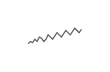
\begin{tikzpicture}[x=0.08em, y=0.08em, line width=0.4pt]
                \draw[FooterGray] (0,3) -- (1,4) -- (2,3.5) -- (3,5) -- (4,4) -- (5,6) -- (6,5.5) -- (7,4) -- (8,5) -- (9,7) -- (10,6) -- (11,5) -- (12,6.5) -- (13,8) -- (14,7) -- (15,6) -- (16,7.5) -- (17,9) -- (18,8) -- (19,7) -- (20,8.5) -- (21,10) -- (22,9) -- (23,8) -- (24,9.5);
            \end{tikzpicture}%
        }%
        \hskip0.5cm%
    }%
    \vskip6pt%
}

%=============================================================================
% PACKAGES
%=============================================================================
\usepackage[utf8]{inputenc}
\DeclareUnicodeCharacter{03B1}{\ensuremath{\alpha}}
\usepackage[T1]{fontenc}
\usepackage{amsmath, amssymb, amsthm}
\usepackage{mathtools}
\usepackage{bm}
\usepackage{tikz}
\usetikzlibrary{arrows.meta, positioning, shapes, calc, decorations.pathreplacing, shadings}
\usepackage{booktabs}
\usepackage{multirow}
\usepackage{array}
\usepackage{graphicx}
\usepackage{animate}
\usepackage{hyperref}
\usepackage{colortbl}
\usepackage{listings}
\lstset{language=Python, basicstyle=\ttfamily\scriptsize, keywordstyle=\color{MainBlue}\bfseries,
  commentstyle=\color{Forest}, stringstyle=\color{Crimson}, breaklines=true,
  frame=none, backgroundcolor=\color{VeryLightGray}, xleftmargin=2mm}
\hypersetup{colorlinks=true, linkcolor=MainBlue, urlcolor=MainBlue}
\graphicspath{{../../logos/}{../../charts/}{../../photos/}}
\usepackage{xcolor}
\hfuzz=2pt  % Suppress tiny overfull warnings (<2pt)
\vfuzz=2pt  % Suppress tiny vertical overfull warnings (<2pt)
% \mathrm in the sans-serif family of the slides (beamer resets \mathrm to the serif family at \begin{document};
% this hook runs after beamer's, so WN, Var, RMSE, ... in formulas match the surrounding text)
% Bold vectors and matrices in the same sans-serif family: \mathbf{A} in sans bold (beamer's own \mathbf came out in
% medium weight), and the bold upright Greek capitals of \boldsymbol / \bm (\bSigma, \bPhi, \boldsymbol{\Theta}) in
% cmss bold: bm.sty fixes its "boldoperators" font when it is loaded (serif cmbx), before beamer switches the
% operators to cmss, so it is reset here.
\AtBeginDocument{%
  \SetMathAlphabet{\mathrm}{normal}{\encodingdefault}{\sfdefault}{\mddefault}{n}%
  \SetMathAlphabet{\mathrm}{bold}{\encodingdefault}{\sfdefault}{bx}{n}%
  \SetMathAlphabet{\mathbf}{normal}{\encodingdefault}{\sfdefault}{bx}{n}%
  \SetMathAlphabet{\mathbf}{bold}{\encodingdefault}{\sfdefault}{bx}{n}%
  \SetSymbolFont{boldoperators}{normal}{OT1}{cmss}{bx}{n}%
  \SetSymbolFont{boldoperators}{bold}{OT1}{cmss}{bx}{n}}

%=============================================================================
% QUANTLET COMMANDS
%   \quantlet{<displayed name>}{<url>}       (generic, compatible with the older TSA decks)
%   \tsaquantlet{Ch_05}{TSA_ch5_garch}       -> https://github.com/danpele/Time-Series-Analysis/tree/main/Quantlets/Ch_05/TSA_ch5_garch
%   \qlurl{<folder>} is defined per chapter by the generator (Quantlets/Ch_NN/<folder>)
%=============================================================================
\newcommand{\tsarepo}{https://github.com/danpele/Time-Series-Analysis}
\newcommand{\tsaqlbase}{https://github.com/danpele/Time-Series-Analysis/tree/main/Quantlets}
\newcommand{\quantlet}[2]{%
    \hfill\href{#2}{%
        \raisebox{-0.15em}{
\includegraphics[height=0.7em]{ql_logo.png}}%
        \textcolor{MainBlue}{\tiny\ #1}%
    }%
}
\newcommand{\tsaquantlet}[2]{\quantlet{\detokenize{#2}}{\tsaqlbase/#1/#2}}

%=============================================================================
% NOTEBOOKS (Google Colab)
%   \colaburl{notebooks/EN/chapter5_seminar_notebook.ipynb} -> the Colab link of a file in the TSA repo
%   \nb: the chapter notebook (each seminar deck redefines it with \renewcommand)
%=============================================================================
\newcommand{\colaburl}[1]{https://colab.research.google.com/github/danpele/Time-Series-Analysis/blob/main/#1}
\newcommand{\nb}{https://colab.research.google.com/github/danpele/Time-Series-Analysis/tree/main/notebooks/EN}
\newcommand{\nbname}{notebooks/EN}

%=============================================================================
% SLIDE HELPERS (used by the generators; the same as in MFM)
%=============================================================================
% local font size for list bodies (the preamble forces \normalsize)
\newcommand{\itemsize}[1]{\setbeamertemplate{itemize/enumerate body begin}{#1}\setbeamertemplate{itemize/enumerate subbody begin}{#1}}
\newcommand{\intitle}[1]{{\hypersetup{urlcolor=white}#1}}   % white links inside coloured title bars
\newcommand{\imgcap}[1]{{\scriptsize #1}\\[0.5mm]}          % caption under a photo
\newcommand{\imgcredit}[2]{{\tiny\color{FooterGray}\href{#1}{#2}}}   % image credit: source URL, author/licence
\newcommand{\aiprompt}[1]{{\ttfamily\color{MainBlue}#1}}     % a prompt to an AI assistant

%=============================================================================
% SEMINARS: student version by default; the instructor wrapper *_solutions.tex sets \solutionstrue
%=============================================================================
\makeatletter\@ifundefined{ifsolutions}{\expandafter\newif\csname ifsolutions\endcsname}{}\makeatother
\newcommand{\solonly}[1]{\ifsolutions #1\fi}
\newcommand{\propsub}{\ifsolutions\else\framesubtitle{\ifdefined\tsalang Rezolvarea se discută la seminar\else Solution discussed in class\fi}\fi}

%=============================================================================
% APPENDIX AND CHAPTER LINKS (latex/appendix_links.py writes the calls; it also re-declares these
% macros before \begin{document}, so the decks compile with or without this preamble block)
%=============================================================================
\providecommand{\tsaapplink}[3]{\hypertarget{#2}{}\hyperlink{#1}{\beamergotobutton{#3}}}
\providecommand{\tsaappback}[2]{\begin{tikzpicture}[remember picture,overlay]\node[anchor=south east] at ([xshift=-3mm,yshift=7mm]current page.south east){\hyperlink{#1}{\beamerreturnbutton{#2}}};\end{tikzpicture}}
\providecommand{\tsachlink}[2]{\href{#1}{#2}}
\providecommand{\tsachlinkt}[2]{\href{#1}{\usebeamercolor[fg]{frametitle}#2}}

%=============================================================================
% QUANTINAR COMMAND: link către un curs Quantinar (subiecte avansate)
%=============================================================================
\newcommand{\quantinar}[2]{%
    \href{#2}{%
        \raisebox{-0.15em}{
\includegraphics[height=0.8em]{qr_logo.png}}%
        \textcolor{MainBlue}{\scriptsize\ #1}%
    }%
}

%=============================================================================
% CUSTOM TITLE PAGE
%=============================================================================
\defbeamertemplate*{title page}{hybrid}[1][]
{
    \vspace{0.2cm}
    % Logos row - top header (with clickable links)
    \begin{center}
        \href{https://www.ase.ro}{
\includegraphics[height=1.0cm]{ase_logo.png}}\hspace{0.3cm}%
        \href{https://theida.net}{
\includegraphics[height=1.0cm]{ida_logo.png}}\hspace{0.3cm}%
        \href{https://blockchain-research-center.com}{
\includegraphics[height=1.0cm]{brc_logo.png}}\hspace{0.3cm}%
        \href{https://www.ai4efin.ase.ro}{
\includegraphics[height=1.0cm]{ai4efin_logo.png}}\hspace{0.3cm}%
        \href{https://ipe.ro/new}{
\includegraphics[height=1.0cm]{acad_logo.png}}\hspace{0.3cm}%
        \href{https://www.digital-finance-msca.com}{
\includegraphics[height=1.0cm]{msca_logo.png}}%
    \end{center}

    \vspace{0.6cm}

    % Main title with Q logos on sides (with clickable links)
    \begin{center}
        \begin{minipage}{0.1\textwidth}
            \centering
            \href{https://quantlet.com}{
\includegraphics[height=1.1cm]{ql_logo.png}}
        \end{minipage}%
        \begin{minipage}{0.78\textwidth}
            \centering
            {\LARGE\bfseries\usebeamercolor[fg]{title}\inserttitle}

            \vspace{0.3cm}

            {\usebeamerfont{subtitle}\usebeamercolor[fg]{title}\insertsubtitle}
        \end{minipage}%
        \begin{minipage}{0.1\textwidth}
            \centering
            \href{https://quantinar.com}{
\includegraphics[height=1.1cm]{qr_logo.png}}
        \end{minipage}
    \end{center}

    \vspace{0.6cm}

    % Authors (left aligned)
    \hspace{0.5cm}{\usebeamerfont{author}\insertauthor}

    \vspace{0.3cm}

    % Institute/Affiliations (left aligned)
    \hspace{0.5cm}\begin{minipage}[t]{0.9\textwidth}
        \raggedright\small\insertinstitute
    \end{minipage}
}

%=============================================================================
% THEOREM ENVIRONMENTS
%=============================================================================
\theoremstyle{definition}
\setbeamertemplate{theorems}[numbered]
\ifdefined\tsalang
\newtheorem{defn}{Definiție}
\newtheorem{thm}{Teoremă}
\newtheorem{prop}{Propoziție}
\newtheorem{rmk}{Observație}
\else
\newtheorem{defn}{Definition}
\newtheorem{thm}{Theorem}
\newtheorem{prop}{Proposition}
\newtheorem{rmk}{Remark}
\fi

%=============================================================================
% CENTRED MINIPAGE (no extra vertical space)
%=============================================================================
\newenvironment{cminipage}[1]{%
    \par\noindent\hfill\begin{minipage}{#1}\ignorespaces
}{%
    \end{minipage}\hfill\null\par
}

%=============================================================================
% CUSTOM COMMANDS
%=============================================================================
\newcommand{\E}{\mathbb{E}}
\newcommand{\Var}{\text{Var}}
\newcommand{\Cov}{\text{Cov}}
\newcommand{\Corr}{\text{Corr}}
\newcommand{\R}{\mathbb{R}}
\newcommand{\N}{\mathbb{N}}
\newcommand{\Z}{\mathbb{Z}}
\newcommand{\B}{\mathbf{B}}
\newcommand{\imark}{\textcolor{MainBlue}{\textbullet}}
\newcommand{\RMSE}{\text{RMSE}}
\newcommand{\MAE}{\text{MAE}}
\newcommand{\MAPE}{\text{MAPE}}

% Boldface vector/matrix commands (VAR, VECM, state space; also used by the older TSA decks)
\newcommand{\bY}{\mathbf{Y}}
\newcommand{\bX}{\mathbf{X}}
\newcommand{\bA}{\mathbf{A}}
\newcommand{\bB}{\mathbf{B}}
\newcommand{\bepsilon}{\boldsymbol{\varepsilon}}
\newcommand{\bSigma}{\boldsymbol{\Sigma}}
\newcommand{\bPhi}{\boldsymbol{\Phi}}
\newcommand{\bGamma}{\boldsymbol{\Gamma}}
\newcommand{\bPi}{\boldsymbol{\Pi}}
\newcommand{\bc}{\mathbf{c}}
\newcommand{\balpha}{\boldsymbol{\alpha}}
\newcommand{\bbeta}{\boldsymbol{\beta}}
\newcommand{\bvarepsilon}{\boldsymbol{\varepsilon}}

% Legacy seminar marks (older TSA seminar decks)
\newcommand{\correct}{\textcolor{Forest}{\checkmark}}
\newcommand{\incorrect}{\textcolor{Crimson}{\texttimes}}
 se definește
%   \newcommand{\coursename}{Time Series Analysis}      (EN)
%   \newcommand{\coursename}{Serii de timp}       (RO)  și  \def\tsalang{ro}
% Fișierele .tex se află în EN/Courses, EN/Seminars, RO/Cursuri, RO/Seminarii (două niveluri sub rădăcină).
% Deck-urile sînt generate de latex/build_chapterN.py / build_seminarN.py (vezi latex/tsa_build.py).

\documentclass[9pt, aspectratio=169, t]{beamer}
\providecommand{\coursename}{Time Series Analysis}

% Ensure content fits on slides
\setbeamersize{text margin left=8mm, text margin right=8mm}
% Smaller institute font (title page)
\setbeamerfont{institute}{size=\footnotesize}

%=============================================================================
% THEME AND STYLE CONFIGURATION
%=============================================================================
\usetheme{default}
% Using default theme for clean header/footer control

% Color Palette (matching Redispatch PDF)
\definecolor{MainBlue}{RGB}{26, 58, 110}
\definecolor{AccentBlue}{RGB}{26, 58, 110}
\definecolor{IDAred}{RGB}{205, 0, 0}
\definecolor{DarkGray}{RGB}{51, 51, 51}
\definecolor{MediumGray}{RGB}{128, 128, 128}
\definecolor{LightGray}{RGB}{248, 248, 248}
\definecolor{VeryLightGray}{RGB}{235, 235, 235}
\definecolor{KeynoteGray}{RGB}{218, 218, 218}
\definecolor{SectionGray}{RGB}{120, 120, 120}
\definecolor{FooterGray}{RGB}{100, 100, 100}
\definecolor{Crimson}{RGB}{220, 53, 69}
\definecolor{Forest}{RGB}{46, 125, 50}
\definecolor{Amber}{RGB}{181, 133, 63}
\definecolor{Orange}{RGB}{230, 126, 34}
\definecolor{Purple}{RGB}{142, 68, 173}

% Gradient background (exact Keynote 315° gradient: white to RGB 218,218,218)
\setbeamertemplate{background}{%
    \begin{tikzpicture}[remember picture, overlay]
        \shade[shading=axis, shading angle=315,
        top color=white, bottom color=KeynoteGray]
        (current page.south west) rectangle (current page.north east);
    \end{tikzpicture}%
}
% Fallback solid color for compatibility
\setbeamercolor{background canvas}{bg=}

\setbeamercolor{palette primary}{bg=MainBlue, fg=white}
\setbeamercolor{palette secondary}{bg=MainBlue!85, fg=white}
\setbeamercolor{palette tertiary}{bg=MainBlue!70, fg=white}
\setbeamercolor{structure}{fg=MainBlue}
\setbeamercolor{title}{fg=IDAred}
\setbeamercolor{frametitle}{fg=IDAred, bg=}
\setbeamercolor{block title}{bg=MainBlue, fg=white}
\setbeamercolor{block body}{bg=VeryLightGray, fg=DarkGray}
\setbeamercolor{block title alerted}{bg=Crimson, fg=white}
\setbeamercolor{block body alerted}{bg=Crimson!8, fg=DarkGray}
\setbeamercolor{block title example}{bg=Forest, fg=white}
\setbeamercolor{block body example}{bg=Forest!8, fg=DarkGray}
\setbeamercolor{item}{fg=MainBlue}

% Footer colors (override Madrid theme blue)
\setbeamercolor{author in head/foot}{fg=FooterGray, bg=}
\setbeamercolor{title in head/foot}{fg=FooterGray, bg=}
\setbeamercolor{date in head/foot}{fg=FooterGray, bg=}
\setbeamercolor{section in head/foot}{fg=FooterGray, bg=}
\setbeamercolor{subsection in head/foot}{fg=FooterGray, bg=}

% Bullet styles (apply everywhere including blocks)
\setbeamertemplate{itemize item}{\color{MainBlue}$\boxdot$}
\setbeamertemplate{itemize subitem}{\color{MainBlue}$\blacktriangleright$}
\setbeamertemplate{itemize subsubitem}{\color{MainBlue}\tiny$\bullet$}
\setbeamertemplate{itemize/enumerate body begin}{\normalsize}
\setbeamertemplate{itemize/enumerate subbody begin}{\normalsize}

% Item spacing - compact style
\setlength{\leftmargini}{10pt}       % Level 1: minimal indent
\setlength{\leftmarginii}{10pt}      % Level 2: minimal additional indent
% Compact list spacing (zero extra space before/after lists in blocks)
\makeatletter
\def\@listi{\leftmargin\leftmargini \topsep 0pt \parsep 0pt \itemsep 0pt}
\def\@listii{\leftmargin\leftmarginii \topsep 0pt \parsep 0pt \itemsep 0pt}
\makeatother

\setbeamertemplate{navigation symbols}{}

%=============================================================================
% CUSTOM HEADLINE
%=============================================================================
\setbeamertemplate{headline}{%
    \vskip10pt%
    \hbox to \paperwidth{%
        \hskip0.5cm%
        {\small\color{FooterGray}\renewcommand{\hyperlink}[2]{##2}\insertsectionhead}%
        \hfill%
        \textcolor{FooterGray}{\small\insertframenumber}%
        \hskip0.5cm%
    }%
    \vskip4pt%
    {\color{FooterGray}\hrule height 0.4pt}%
}

%=============================================================================
% CUSTOM FOOTER
%=============================================================================
\usepackage{fontawesome5}

\setbeamertemplate{footline}{%
    {\color{FooterGray}\hrule height 0.4pt}%
    \vskip4pt%
    \hbox to \paperwidth{%
        \hskip0.5cm%
        \textcolor{FooterGray}{\small\coursename}%
        \hfill%
        \raisebox{-0.1em}{%
            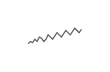
\begin{tikzpicture}[x=0.08em, y=0.08em, line width=0.4pt]
                \draw[FooterGray] (0,3) -- (1,4) -- (2,3.5) -- (3,5) -- (4,4) -- (5,6) -- (6,5.5) -- (7,4) -- (8,5) -- (9,7) -- (10,6) -- (11,5) -- (12,6.5) -- (13,8) -- (14,7) -- (15,6) -- (16,7.5) -- (17,9) -- (18,8) -- (19,7) -- (20,8.5) -- (21,10) -- (22,9) -- (23,8) -- (24,9.5);
            \end{tikzpicture}%
        }%
        \hskip0.5cm%
    }%
    \vskip6pt%
}

%=============================================================================
% PACKAGES
%=============================================================================
\usepackage[utf8]{inputenc}
\DeclareUnicodeCharacter{03B1}{\ensuremath{\alpha}}
\usepackage[T1]{fontenc}
\usepackage{amsmath, amssymb, amsthm}
\usepackage{mathtools}
\usepackage{bm}
\usepackage{tikz}
\usetikzlibrary{arrows.meta, positioning, shapes, calc, decorations.pathreplacing, shadings}
\usepackage{booktabs}
\usepackage{multirow}
\usepackage{array}
\usepackage{graphicx}
\usepackage{animate}
\usepackage{hyperref}
\usepackage{colortbl}
\usepackage{listings}
\lstset{language=Python, basicstyle=\ttfamily\scriptsize, keywordstyle=\color{MainBlue}\bfseries,
  commentstyle=\color{Forest}, stringstyle=\color{Crimson}, breaklines=true,
  frame=none, backgroundcolor=\color{VeryLightGray}, xleftmargin=2mm}
\hypersetup{colorlinks=true, linkcolor=MainBlue, urlcolor=MainBlue}
\graphicspath{{../../logos/}{../../charts/}{../../photos/}}
\usepackage{xcolor}
\hfuzz=2pt  % Suppress tiny overfull warnings (<2pt)
\vfuzz=2pt  % Suppress tiny vertical overfull warnings (<2pt)
% \mathrm in the sans-serif family of the slides (beamer resets \mathrm to the serif family at \begin{document};
% this hook runs after beamer's, so WN, Var, RMSE, ... in formulas match the surrounding text)
% Bold vectors and matrices in the same sans-serif family: \mathbf{A} in sans bold (beamer's own \mathbf came out in
% medium weight), and the bold upright Greek capitals of \boldsymbol / \bm (\bSigma, \bPhi, \boldsymbol{\Theta}) in
% cmss bold: bm.sty fixes its "boldoperators" font when it is loaded (serif cmbx), before beamer switches the
% operators to cmss, so it is reset here.
\AtBeginDocument{%
  \SetMathAlphabet{\mathrm}{normal}{\encodingdefault}{\sfdefault}{\mddefault}{n}%
  \SetMathAlphabet{\mathrm}{bold}{\encodingdefault}{\sfdefault}{bx}{n}%
  \SetMathAlphabet{\mathbf}{normal}{\encodingdefault}{\sfdefault}{bx}{n}%
  \SetMathAlphabet{\mathbf}{bold}{\encodingdefault}{\sfdefault}{bx}{n}%
  \SetSymbolFont{boldoperators}{normal}{OT1}{cmss}{bx}{n}%
  \SetSymbolFont{boldoperators}{bold}{OT1}{cmss}{bx}{n}}

%=============================================================================
% QUANTLET COMMANDS
%   \quantlet{<displayed name>}{<url>}       (generic, compatible with the older TSA decks)
%   \tsaquantlet{Ch_05}{TSA_ch5_garch}       -> https://github.com/danpele/Time-Series-Analysis/tree/main/Quantlets/Ch_05/TSA_ch5_garch
%   \qlurl{<folder>} is defined per chapter by the generator (Quantlets/Ch_NN/<folder>)
%=============================================================================
\newcommand{\tsarepo}{https://github.com/danpele/Time-Series-Analysis}
\newcommand{\tsaqlbase}{https://github.com/danpele/Time-Series-Analysis/tree/main/Quantlets}
\newcommand{\quantlet}[2]{%
    \hfill\href{#2}{%
        \raisebox{-0.15em}{
\includegraphics[height=0.7em]{ql_logo.png}}%
        \textcolor{MainBlue}{\tiny\ #1}%
    }%
}
\newcommand{\tsaquantlet}[2]{\quantlet{\detokenize{#2}}{\tsaqlbase/#1/#2}}

%=============================================================================
% NOTEBOOKS (Google Colab)
%   \colaburl{notebooks/EN/chapter5_seminar_notebook.ipynb} -> the Colab link of a file in the TSA repo
%   \nb: the chapter notebook (each seminar deck redefines it with \renewcommand)
%=============================================================================
\newcommand{\colaburl}[1]{https://colab.research.google.com/github/danpele/Time-Series-Analysis/blob/main/#1}
\newcommand{\nb}{https://colab.research.google.com/github/danpele/Time-Series-Analysis/tree/main/notebooks/EN}
\newcommand{\nbname}{notebooks/EN}

%=============================================================================
% SLIDE HELPERS (used by the generators; the same as in MFM)
%=============================================================================
% local font size for list bodies (the preamble forces \normalsize)
\newcommand{\itemsize}[1]{\setbeamertemplate{itemize/enumerate body begin}{#1}\setbeamertemplate{itemize/enumerate subbody begin}{#1}}
\newcommand{\intitle}[1]{{\hypersetup{urlcolor=white}#1}}   % white links inside coloured title bars
\newcommand{\imgcap}[1]{{\scriptsize #1}\\[0.5mm]}          % caption under a photo
\newcommand{\imgcredit}[2]{{\tiny\color{FooterGray}\href{#1}{#2}}}   % image credit: source URL, author/licence
\newcommand{\aiprompt}[1]{{\ttfamily\color{MainBlue}#1}}     % a prompt to an AI assistant

%=============================================================================
% SEMINARS: student version by default; the instructor wrapper *_solutions.tex sets \solutionstrue
%=============================================================================
\makeatletter\@ifundefined{ifsolutions}{\expandafter\newif\csname ifsolutions\endcsname}{}\makeatother
\newcommand{\solonly}[1]{\ifsolutions #1\fi}
\newcommand{\propsub}{\ifsolutions\else\framesubtitle{\ifdefined\tsalang Rezolvarea se discută la seminar\else Solution discussed in class\fi}\fi}

%=============================================================================
% APPENDIX AND CHAPTER LINKS (latex/appendix_links.py writes the calls; it also re-declares these
% macros before \begin{document}, so the decks compile with or without this preamble block)
%=============================================================================
\providecommand{\tsaapplink}[3]{\hypertarget{#2}{}\hyperlink{#1}{\beamergotobutton{#3}}}
\providecommand{\tsaappback}[2]{\begin{tikzpicture}[remember picture,overlay]\node[anchor=south east] at ([xshift=-3mm,yshift=7mm]current page.south east){\hyperlink{#1}{\beamerreturnbutton{#2}}};\end{tikzpicture}}
\providecommand{\tsachlink}[2]{\href{#1}{#2}}
\providecommand{\tsachlinkt}[2]{\href{#1}{\usebeamercolor[fg]{frametitle}#2}}

%=============================================================================
% QUANTINAR COMMAND: link către un curs Quantinar (subiecte avansate)
%=============================================================================
\newcommand{\quantinar}[2]{%
    \href{#2}{%
        \raisebox{-0.15em}{
\includegraphics[height=0.8em]{qr_logo.png}}%
        \textcolor{MainBlue}{\scriptsize\ #1}%
    }%
}

%=============================================================================
% CUSTOM TITLE PAGE
%=============================================================================
\defbeamertemplate*{title page}{hybrid}[1][]
{
    \vspace{0.2cm}
    % Logos row - top header (with clickable links)
    \begin{center}
        \href{https://www.ase.ro}{
\includegraphics[height=1.0cm]{ase_logo.png}}\hspace{0.3cm}%
        \href{https://theida.net}{
\includegraphics[height=1.0cm]{ida_logo.png}}\hspace{0.3cm}%
        \href{https://blockchain-research-center.com}{
\includegraphics[height=1.0cm]{brc_logo.png}}\hspace{0.3cm}%
        \href{https://www.ai4efin.ase.ro}{
\includegraphics[height=1.0cm]{ai4efin_logo.png}}\hspace{0.3cm}%
        \href{https://ipe.ro/new}{
\includegraphics[height=1.0cm]{acad_logo.png}}\hspace{0.3cm}%
        \href{https://www.digital-finance-msca.com}{
\includegraphics[height=1.0cm]{msca_logo.png}}%
    \end{center}

    \vspace{0.6cm}

    % Main title with Q logos on sides (with clickable links)
    \begin{center}
        \begin{minipage}{0.1\textwidth}
            \centering
            \href{https://quantlet.com}{
\includegraphics[height=1.1cm]{ql_logo.png}}
        \end{minipage}%
        \begin{minipage}{0.78\textwidth}
            \centering
            {\LARGE\bfseries\usebeamercolor[fg]{title}\inserttitle}

            \vspace{0.3cm}

            {\usebeamerfont{subtitle}\usebeamercolor[fg]{title}\insertsubtitle}
        \end{minipage}%
        \begin{minipage}{0.1\textwidth}
            \centering
            \href{https://quantinar.com}{
\includegraphics[height=1.1cm]{qr_logo.png}}
        \end{minipage}
    \end{center}

    \vspace{0.6cm}

    % Authors (left aligned)
    \hspace{0.5cm}{\usebeamerfont{author}\insertauthor}

    \vspace{0.3cm}

    % Institute/Affiliations (left aligned)
    \hspace{0.5cm}\begin{minipage}[t]{0.9\textwidth}
        \raggedright\small\insertinstitute
    \end{minipage}
}

%=============================================================================
% THEOREM ENVIRONMENTS
%=============================================================================
\theoremstyle{definition}
\setbeamertemplate{theorems}[numbered]
\ifdefined\tsalang
\newtheorem{defn}{Definiție}
\newtheorem{thm}{Teoremă}
\newtheorem{prop}{Propoziție}
\newtheorem{rmk}{Observație}
\else
\newtheorem{defn}{Definition}
\newtheorem{thm}{Theorem}
\newtheorem{prop}{Proposition}
\newtheorem{rmk}{Remark}
\fi

%=============================================================================
% CENTRED MINIPAGE (no extra vertical space)
%=============================================================================
\newenvironment{cminipage}[1]{%
    \par\noindent\hfill\begin{minipage}{#1}\ignorespaces
}{%
    \end{minipage}\hfill\null\par
}

%=============================================================================
% CUSTOM COMMANDS
%=============================================================================
\newcommand{\E}{\mathbb{E}}
\newcommand{\Var}{\text{Var}}
\newcommand{\Cov}{\text{Cov}}
\newcommand{\Corr}{\text{Corr}}
\newcommand{\R}{\mathbb{R}}
\newcommand{\N}{\mathbb{N}}
\newcommand{\Z}{\mathbb{Z}}
\newcommand{\B}{\mathbf{B}}
\newcommand{\imark}{\textcolor{MainBlue}{\textbullet}}
\newcommand{\RMSE}{\text{RMSE}}
\newcommand{\MAE}{\text{MAE}}
\newcommand{\MAPE}{\text{MAPE}}

% Boldface vector/matrix commands (VAR, VECM, state space; also used by the older TSA decks)
\newcommand{\bY}{\mathbf{Y}}
\newcommand{\bX}{\mathbf{X}}
\newcommand{\bA}{\mathbf{A}}
\newcommand{\bB}{\mathbf{B}}
\newcommand{\bepsilon}{\boldsymbol{\varepsilon}}
\newcommand{\bSigma}{\boldsymbol{\Sigma}}
\newcommand{\bPhi}{\boldsymbol{\Phi}}
\newcommand{\bGamma}{\boldsymbol{\Gamma}}
\newcommand{\bPi}{\boldsymbol{\Pi}}
\newcommand{\bc}{\mathbf{c}}
\newcommand{\balpha}{\boldsymbol{\alpha}}
\newcommand{\bbeta}{\boldsymbol{\beta}}
\newcommand{\bvarepsilon}{\boldsymbol{\varepsilon}}

% Legacy seminar marks (older TSA seminar decks)
\newcommand{\correct}{\textcolor{Forest}{\checkmark}}
\newcommand{\incorrect}{\textcolor{Crimson}{\texttimes}}
 se definește
%   \newcommand{\coursename}{Time Series Analysis}      (EN)
%   \newcommand{\coursename}{Serii de timp}       (RO)  și  \def\tsalang{ro}
% Fișierele .tex se află în EN/Courses, EN/Seminars, RO/Cursuri, RO/Seminarii (două niveluri sub rădăcină).
% Deck-urile sînt generate de latex/build_chapterN.py / build_seminarN.py (vezi latex/tsa_build.py).

\documentclass[9pt, aspectratio=169, t]{beamer}
\providecommand{\coursename}{Time Series Analysis}

% Ensure content fits on slides
\setbeamersize{text margin left=8mm, text margin right=8mm}
% Smaller institute font (title page)
\setbeamerfont{institute}{size=\footnotesize}

%=============================================================================
% THEME AND STYLE CONFIGURATION
%=============================================================================
\usetheme{default}
% Using default theme for clean header/footer control

% Color Palette (matching Redispatch PDF)
\definecolor{MainBlue}{RGB}{26, 58, 110}
\definecolor{AccentBlue}{RGB}{26, 58, 110}
\definecolor{IDAred}{RGB}{205, 0, 0}
\definecolor{DarkGray}{RGB}{51, 51, 51}
\definecolor{MediumGray}{RGB}{128, 128, 128}
\definecolor{LightGray}{RGB}{248, 248, 248}
\definecolor{VeryLightGray}{RGB}{235, 235, 235}
\definecolor{KeynoteGray}{RGB}{218, 218, 218}
\definecolor{SectionGray}{RGB}{120, 120, 120}
\definecolor{FooterGray}{RGB}{100, 100, 100}
\definecolor{Crimson}{RGB}{220, 53, 69}
\definecolor{Forest}{RGB}{46, 125, 50}
\definecolor{Amber}{RGB}{181, 133, 63}
\definecolor{Orange}{RGB}{230, 126, 34}
\definecolor{Purple}{RGB}{142, 68, 173}

% Gradient background (exact Keynote 315° gradient: white to RGB 218,218,218)
\setbeamertemplate{background}{%
    \begin{tikzpicture}[remember picture, overlay]
        \shade[shading=axis, shading angle=315,
        top color=white, bottom color=KeynoteGray]
        (current page.south west) rectangle (current page.north east);
    \end{tikzpicture}%
}
% Fallback solid color for compatibility
\setbeamercolor{background canvas}{bg=}

\setbeamercolor{palette primary}{bg=MainBlue, fg=white}
\setbeamercolor{palette secondary}{bg=MainBlue!85, fg=white}
\setbeamercolor{palette tertiary}{bg=MainBlue!70, fg=white}
\setbeamercolor{structure}{fg=MainBlue}
\setbeamercolor{title}{fg=IDAred}
\setbeamercolor{frametitle}{fg=IDAred, bg=}
\setbeamercolor{block title}{bg=MainBlue, fg=white}
\setbeamercolor{block body}{bg=VeryLightGray, fg=DarkGray}
\setbeamercolor{block title alerted}{bg=Crimson, fg=white}
\setbeamercolor{block body alerted}{bg=Crimson!8, fg=DarkGray}
\setbeamercolor{block title example}{bg=Forest, fg=white}
\setbeamercolor{block body example}{bg=Forest!8, fg=DarkGray}
\setbeamercolor{item}{fg=MainBlue}

% Footer colors (override Madrid theme blue)
\setbeamercolor{author in head/foot}{fg=FooterGray, bg=}
\setbeamercolor{title in head/foot}{fg=FooterGray, bg=}
\setbeamercolor{date in head/foot}{fg=FooterGray, bg=}
\setbeamercolor{section in head/foot}{fg=FooterGray, bg=}
\setbeamercolor{subsection in head/foot}{fg=FooterGray, bg=}

% Bullet styles (apply everywhere including blocks)
\setbeamertemplate{itemize item}{\color{MainBlue}$\boxdot$}
\setbeamertemplate{itemize subitem}{\color{MainBlue}$\blacktriangleright$}
\setbeamertemplate{itemize subsubitem}{\color{MainBlue}\tiny$\bullet$}
\setbeamertemplate{itemize/enumerate body begin}{\normalsize}
\setbeamertemplate{itemize/enumerate subbody begin}{\normalsize}

% Item spacing - compact style
\setlength{\leftmargini}{10pt}       % Level 1: minimal indent
\setlength{\leftmarginii}{10pt}      % Level 2: minimal additional indent
% Compact list spacing (zero extra space before/after lists in blocks)
\makeatletter
\def\@listi{\leftmargin\leftmargini \topsep 0pt \parsep 0pt \itemsep 0pt}
\def\@listii{\leftmargin\leftmarginii \topsep 0pt \parsep 0pt \itemsep 0pt}
\makeatother

\setbeamertemplate{navigation symbols}{}

%=============================================================================
% CUSTOM HEADLINE
%=============================================================================
\setbeamertemplate{headline}{%
    \vskip10pt%
    \hbox to \paperwidth{%
        \hskip0.5cm%
        {\small\color{FooterGray}\renewcommand{\hyperlink}[2]{##2}\insertsectionhead}%
        \hfill%
        \textcolor{FooterGray}{\small\insertframenumber}%
        \hskip0.5cm%
    }%
    \vskip4pt%
    {\color{FooterGray}\hrule height 0.4pt}%
}

%=============================================================================
% CUSTOM FOOTER
%=============================================================================
\usepackage{fontawesome5}

\setbeamertemplate{footline}{%
    {\color{FooterGray}\hrule height 0.4pt}%
    \vskip4pt%
    \hbox to \paperwidth{%
        \hskip0.5cm%
        \textcolor{FooterGray}{\small\coursename}%
        \hfill%
        \raisebox{-0.1em}{%
            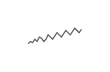
\begin{tikzpicture}[x=0.08em, y=0.08em, line width=0.4pt]
                \draw[FooterGray] (0,3) -- (1,4) -- (2,3.5) -- (3,5) -- (4,4) -- (5,6) -- (6,5.5) -- (7,4) -- (8,5) -- (9,7) -- (10,6) -- (11,5) -- (12,6.5) -- (13,8) -- (14,7) -- (15,6) -- (16,7.5) -- (17,9) -- (18,8) -- (19,7) -- (20,8.5) -- (21,10) -- (22,9) -- (23,8) -- (24,9.5);
            \end{tikzpicture}%
        }%
        \hskip0.5cm%
    }%
    \vskip6pt%
}

%=============================================================================
% PACKAGES
%=============================================================================
\usepackage[utf8]{inputenc}
\DeclareUnicodeCharacter{03B1}{\ensuremath{\alpha}}
\usepackage[T1]{fontenc}
\usepackage{amsmath, amssymb, amsthm}
\usepackage{mathtools}
\usepackage{bm}
\usepackage{tikz}
\usetikzlibrary{arrows.meta, positioning, shapes, calc, decorations.pathreplacing, shadings}
\usepackage{booktabs}
\usepackage{multirow}
\usepackage{array}
\usepackage{graphicx}
\usepackage{animate}
\usepackage{hyperref}
\usepackage{colortbl}
\usepackage{listings}
\lstset{language=Python, basicstyle=\ttfamily\scriptsize, keywordstyle=\color{MainBlue}\bfseries,
  commentstyle=\color{Forest}, stringstyle=\color{Crimson}, breaklines=true,
  frame=none, backgroundcolor=\color{VeryLightGray}, xleftmargin=2mm}
\hypersetup{colorlinks=true, linkcolor=MainBlue, urlcolor=MainBlue}
\graphicspath{{../../logos/}{../../charts/}{../../photos/}}
\usepackage{xcolor}
\hfuzz=2pt  % Suppress tiny overfull warnings (<2pt)
\vfuzz=2pt  % Suppress tiny vertical overfull warnings (<2pt)
% \mathrm in the sans-serif family of the slides (beamer resets \mathrm to the serif family at \begin{document};
% this hook runs after beamer's, so WN, Var, RMSE, ... in formulas match the surrounding text)
% Bold vectors and matrices in the same sans-serif family: \mathbf{A} in sans bold (beamer's own \mathbf came out in
% medium weight), and the bold upright Greek capitals of \boldsymbol / \bm (\bSigma, \bPhi, \boldsymbol{\Theta}) in
% cmss bold: bm.sty fixes its "boldoperators" font when it is loaded (serif cmbx), before beamer switches the
% operators to cmss, so it is reset here.
\AtBeginDocument{%
  \SetMathAlphabet{\mathrm}{normal}{\encodingdefault}{\sfdefault}{\mddefault}{n}%
  \SetMathAlphabet{\mathrm}{bold}{\encodingdefault}{\sfdefault}{bx}{n}%
  \SetMathAlphabet{\mathbf}{normal}{\encodingdefault}{\sfdefault}{bx}{n}%
  \SetMathAlphabet{\mathbf}{bold}{\encodingdefault}{\sfdefault}{bx}{n}%
  \SetSymbolFont{boldoperators}{normal}{OT1}{cmss}{bx}{n}%
  \SetSymbolFont{boldoperators}{bold}{OT1}{cmss}{bx}{n}}

%=============================================================================
% QUANTLET COMMANDS
%   \quantlet{<displayed name>}{<url>}       (generic, compatible with the older TSA decks)
%   \tsaquantlet{Ch_05}{TSA_ch5_garch}       -> https://github.com/danpele/Time-Series-Analysis/tree/main/Quantlets/Ch_05/TSA_ch5_garch
%   \qlurl{<folder>} is defined per chapter by the generator (Quantlets/Ch_NN/<folder>)
%=============================================================================
\newcommand{\tsarepo}{https://github.com/danpele/Time-Series-Analysis}
\newcommand{\tsaqlbase}{https://github.com/danpele/Time-Series-Analysis/tree/main/Quantlets}
\newcommand{\quantlet}[2]{%
    \hfill\href{#2}{%
        \raisebox{-0.15em}{
\includegraphics[height=0.7em]{ql_logo.png}}%
        \textcolor{MainBlue}{\tiny\ #1}%
    }%
}
\newcommand{\tsaquantlet}[2]{\quantlet{\detokenize{#2}}{\tsaqlbase/#1/#2}}

%=============================================================================
% NOTEBOOKS (Google Colab)
%   \colaburl{notebooks/EN/chapter5_seminar_notebook.ipynb} -> the Colab link of a file in the TSA repo
%   \nb: the chapter notebook (each seminar deck redefines it with \renewcommand)
%=============================================================================
\newcommand{\colaburl}[1]{https://colab.research.google.com/github/danpele/Time-Series-Analysis/blob/main/#1}
\newcommand{\nb}{https://colab.research.google.com/github/danpele/Time-Series-Analysis/tree/main/notebooks/EN}
\newcommand{\nbname}{notebooks/EN}

%=============================================================================
% SLIDE HELPERS (used by the generators; the same as in MFM)
%=============================================================================
% local font size for list bodies (the preamble forces \normalsize)
\newcommand{\itemsize}[1]{\setbeamertemplate{itemize/enumerate body begin}{#1}\setbeamertemplate{itemize/enumerate subbody begin}{#1}}
\newcommand{\intitle}[1]{{\hypersetup{urlcolor=white}#1}}   % white links inside coloured title bars
\newcommand{\imgcap}[1]{{\scriptsize #1}\\[0.5mm]}          % caption under a photo
\newcommand{\imgcredit}[2]{{\tiny\color{FooterGray}\href{#1}{#2}}}   % image credit: source URL, author/licence
\newcommand{\aiprompt}[1]{{\ttfamily\color{MainBlue}#1}}     % a prompt to an AI assistant

%=============================================================================
% SEMINARS: student version by default; the instructor wrapper *_solutions.tex sets \solutionstrue
%=============================================================================
\makeatletter\@ifundefined{ifsolutions}{\expandafter\newif\csname ifsolutions\endcsname}{}\makeatother
\newcommand{\solonly}[1]{\ifsolutions #1\fi}
\newcommand{\propsub}{\ifsolutions\else\framesubtitle{\ifdefined\tsalang Rezolvarea se discută la seminar\else Solution discussed in class\fi}\fi}

%=============================================================================
% APPENDIX AND CHAPTER LINKS (latex/appendix_links.py writes the calls; it also re-declares these
% macros before \begin{document}, so the decks compile with or without this preamble block)
%=============================================================================
\providecommand{\tsaapplink}[3]{\hypertarget{#2}{}\hyperlink{#1}{\beamergotobutton{#3}}}
\providecommand{\tsaappback}[2]{\begin{tikzpicture}[remember picture,overlay]\node[anchor=south east] at ([xshift=-3mm,yshift=7mm]current page.south east){\hyperlink{#1}{\beamerreturnbutton{#2}}};\end{tikzpicture}}
\providecommand{\tsachlink}[2]{\href{#1}{#2}}
\providecommand{\tsachlinkt}[2]{\href{#1}{\usebeamercolor[fg]{frametitle}#2}}

%=============================================================================
% QUANTINAR COMMAND: link către un curs Quantinar (subiecte avansate)
%=============================================================================
\newcommand{\quantinar}[2]{%
    \href{#2}{%
        \raisebox{-0.15em}{
\includegraphics[height=0.8em]{qr_logo.png}}%
        \textcolor{MainBlue}{\scriptsize\ #1}%
    }%
}

%=============================================================================
% CUSTOM TITLE PAGE
%=============================================================================
\defbeamertemplate*{title page}{hybrid}[1][]
{
    \vspace{0.2cm}
    % Logos row - top header (with clickable links)
    \begin{center}
        \href{https://www.ase.ro}{
\includegraphics[height=1.0cm]{ase_logo.png}}\hspace{0.3cm}%
        \href{https://theida.net}{
\includegraphics[height=1.0cm]{ida_logo.png}}\hspace{0.3cm}%
        \href{https://blockchain-research-center.com}{
\includegraphics[height=1.0cm]{brc_logo.png}}\hspace{0.3cm}%
        \href{https://www.ai4efin.ase.ro}{
\includegraphics[height=1.0cm]{ai4efin_logo.png}}\hspace{0.3cm}%
        \href{https://ipe.ro/new}{
\includegraphics[height=1.0cm]{acad_logo.png}}\hspace{0.3cm}%
        \href{https://www.digital-finance-msca.com}{
\includegraphics[height=1.0cm]{msca_logo.png}}%
    \end{center}

    \vspace{0.6cm}

    % Main title with Q logos on sides (with clickable links)
    \begin{center}
        \begin{minipage}{0.1\textwidth}
            \centering
            \href{https://quantlet.com}{
\includegraphics[height=1.1cm]{ql_logo.png}}
        \end{minipage}%
        \begin{minipage}{0.78\textwidth}
            \centering
            {\LARGE\bfseries\usebeamercolor[fg]{title}\inserttitle}

            \vspace{0.3cm}

            {\usebeamerfont{subtitle}\usebeamercolor[fg]{title}\insertsubtitle}
        \end{minipage}%
        \begin{minipage}{0.1\textwidth}
            \centering
            \href{https://quantinar.com}{
\includegraphics[height=1.1cm]{qr_logo.png}}
        \end{minipage}
    \end{center}

    \vspace{0.6cm}

    % Authors (left aligned)
    \hspace{0.5cm}{\usebeamerfont{author}\insertauthor}

    \vspace{0.3cm}

    % Institute/Affiliations (left aligned)
    \hspace{0.5cm}\begin{minipage}[t]{0.9\textwidth}
        \raggedright\small\insertinstitute
    \end{minipage}
}

%=============================================================================
% THEOREM ENVIRONMENTS
%=============================================================================
\theoremstyle{definition}
\setbeamertemplate{theorems}[numbered]
\ifdefined\tsalang
\newtheorem{defn}{Definiție}
\newtheorem{thm}{Teoremă}
\newtheorem{prop}{Propoziție}
\newtheorem{rmk}{Observație}
\else
\newtheorem{defn}{Definition}
\newtheorem{thm}{Theorem}
\newtheorem{prop}{Proposition}
\newtheorem{rmk}{Remark}
\fi

%=============================================================================
% CENTRED MINIPAGE (no extra vertical space)
%=============================================================================
\newenvironment{cminipage}[1]{%
    \par\noindent\hfill\begin{minipage}{#1}\ignorespaces
}{%
    \end{minipage}\hfill\null\par
}

%=============================================================================
% CUSTOM COMMANDS
%=============================================================================
\newcommand{\E}{\mathbb{E}}
\newcommand{\Var}{\text{Var}}
\newcommand{\Cov}{\text{Cov}}
\newcommand{\Corr}{\text{Corr}}
\newcommand{\R}{\mathbb{R}}
\newcommand{\N}{\mathbb{N}}
\newcommand{\Z}{\mathbb{Z}}
\newcommand{\B}{\mathbf{B}}
\newcommand{\imark}{\textcolor{MainBlue}{\textbullet}}
\newcommand{\RMSE}{\text{RMSE}}
\newcommand{\MAE}{\text{MAE}}
\newcommand{\MAPE}{\text{MAPE}}

% Boldface vector/matrix commands (VAR, VECM, state space; also used by the older TSA decks)
\newcommand{\bY}{\mathbf{Y}}
\newcommand{\bX}{\mathbf{X}}
\newcommand{\bA}{\mathbf{A}}
\newcommand{\bB}{\mathbf{B}}
\newcommand{\bepsilon}{\boldsymbol{\varepsilon}}
\newcommand{\bSigma}{\boldsymbol{\Sigma}}
\newcommand{\bPhi}{\boldsymbol{\Phi}}
\newcommand{\bGamma}{\boldsymbol{\Gamma}}
\newcommand{\bPi}{\boldsymbol{\Pi}}
\newcommand{\bc}{\mathbf{c}}
\newcommand{\balpha}{\boldsymbol{\alpha}}
\newcommand{\bbeta}{\boldsymbol{\beta}}
\newcommand{\bvarepsilon}{\boldsymbol{\varepsilon}}

% Legacy seminar marks (older TSA seminar decks)
\newcommand{\correct}{\textcolor{Forest}{\checkmark}}
\newcommand{\incorrect}{\textcolor{Crimson}{\texttimes}}


\newcommand{\qlurl}[1]{https://github.com/danpele/Time-Series-Analysis/tree/main/Quantlets/Ch_06/#1}

% Clickable citations (DOIs verified via Crossref)
\newcommand{\refHP}{\href{https://doi.org/10.1007/978-3-031-13584-2}{Huang și Petukhina (2022)}}
\newcommand{\refFPP}{\href{https://otexts.com/fpp3/VAR.html}{Hyndman și Athanasopoulos (2021)}}
\newcommand{\refLut}{\href{https://doi.org/10.1007/978-3-540-27752-1}{Lütkepohl (2005)}}
\newcommand{\refHamilton}{\href{https://doi.org/10.2307/j.ctv14jx6sm}{Hamilton (1994)}}
\newcommand{\refSims}{\href{https://doi.org/10.2307/1912017}{Sims (1980)}}
\newcommand{\refSimsPP}{\href{https://doi.org/10.1016/0014-2921(92)90041-T}{Sims (1992)}}
\newcommand{\refGranger}{\href{https://doi.org/10.2307/1912791}{Granger (1969)}}
\newcommand{\refLutOm}{\href{https://doi.org/10.1016/0304-4076(82)90011-2}{Lütkepohl (1982)}}
\newcommand{\refTY}{\href{https://doi.org/10.1016/0304-4076(94)01616-8}{Toda și Yamamoto (1995)}}
\newcommand{\refSSW}{\href{https://doi.org/10.2307/2938337}{Sims, Stock și Watson (1990)}}
\newcommand{\refSW}{\href{https://doi.org/10.1257/jep.15.4.101}{Stock și Watson (2001)}}
\newcommand{\refPS}{\href{https://doi.org/10.1016/S0165-1765(97)00214-0}{Pesaran și Shin (1998)}}
\newcommand{\refKPP}{\href{https://doi.org/10.1016/0304-4076(95)01753-4}{Koop, Pesaran și Potter (1996)}}
\newcommand{\refDY}{\href{https://doi.org/10.1111/j.1468-0297.2008.02208.x}{Diebold și Yilmaz (2009)}}
\newcommand{\refDYb}{\href{https://doi.org/10.1016/j.ijforecast.2011.02.006}{Diebold și Yilmaz (2012)}}
\newcommand{\refKilian}{\href{https://doi.org/10.1162/003465398557465}{Kilian (1998)}}
\newcommand{\refHosking}{\href{https://doi.org/10.1080/01621459.1980.10477520}{Hosking (1980)}}
\newcommand{\refJB}{\href{https://doi.org/10.1016/0165-1765(80)90024-5}{Jarque și Bera (1980)}}
\newcommand{\refAkaike}{\href{https://doi.org/10.1109/TAC.1974.1100705}{Akaike (1974)}}
\newcommand{\refSchwarz}{\href{https://doi.org/10.1214/aos/1176344136}{Schwarz (1978)}}
\newcommand{\refHQ}{\href{https://doi.org/10.1111/j.2517-6161.1979.tb01072.x}{Hannan și Quinn (1979)}}
\newcommand{\refDM}{\href{https://doi.org/10.1080/07350015.1995.10524599}{Diebold și Mariano (1995)}}
\newcommand{\refEG}{\href{https://doi.org/10.2307/1913236}{Engle și Granger (1987)}}

\title[Serii de timp]{Serii de timp}
\subtitle{Capitolul 6: Modele VAR și cauzalitate Granger}
\author[D.T. Pele]{Daniel Traian PELE}
\institute{Academia de Studii Economice din București\\
IDA Institute Digital Assets\\
Blockchain Research Center\\
AI4EFin Artificial Intelligence for Energy Finance\\
Academia Română, Institutul de Prognoză Economică\\
MSCA Digital Finance}
\date{}

%=============================================================================
\providecommand{\tsaapplink}[3]{\hypertarget{#2}{}\hyperlink{#1}{\beamergotobutton{#3}}}  % APPLINKS-MACROS
\providecommand{\tsaappback}[2]{\begin{tikzpicture}[remember picture,overlay]\node[anchor=south east] at ([xshift=-3mm,yshift=7mm]current page.south east){\hyperlink{#1}{\beamerreturnbutton{#2}}};\end{tikzpicture}}  % APPLINKS-MACROS
\providecommand{\tsachlink}[2]{\href{#1}{#2}}  % APPLINKS-MACROS
\providecommand{\tsachlinkt}[2]{\href{#1}{\usebeamercolor[fg]{frametitle}#2}}  % APPLINKS-MACROS
\begin{document}
%=============================================================================

{
\setbeamertemplate{headline}{}
\setbeamertemplate{footline}{}
\begin{frame}[noframenumbering]
    \titlepage
\end{frame}
}
% BEGIN-ACRONYMS (generat de latex/acronyms.py; nu editati manual)
\begin{frame}{Acronime folosite în acest material (1/2)}
\setbeamertemplate{itemize/enumerate body begin}{\tiny}
\begin{columns}[T]
\begin{column}{0.49\textwidth}
\begin{itemize}\setlength{\itemsep}{0pt}
    \item \textbf{AI}: Artificial Intelligence (inteligență artificială)
    \item \textbf{AIC}: Akaike Information Criterion (criteriul informațional Akaike)
    \item \textbf{AR}: AutoRegressive (model); in event studies: Abnormal Return (model autoregresiv; în studiile de eveniment: randament anormal)
    \item \textbf{ARMA}: AutoRegressive Moving Average (model) — model autoregresiv cu medie mobilă
    \item \textbf{BET}: Bucharest Exchange Trading (index) — indicele de referință al Bursei de Valori București
    \item \textbf{BIC}: Bayesian Information Criterion (criteriul informațional bayesian (Schwarz))
    \item \textbf{BNR}: Banca Națională a României
    \item \textbf{CCF}: Cross-Correlation Function (funcția de corelație încrucișată)
    \item \textbf{COVID-19}: COronaVIrus Disease 2019 (boala provocată de coronavirus, 2019)
    \item \textbf{DM}: Diebold–Mariano (test) — testul Diebold–Mariano de comparare a prognozelor
    \item \textbf{DSGE}: Dynamic Stochastic General Equilibrium (model) — model dinamic stochastic de echilibru general
    \item \textbf{EODHD}: EOD Historical Data (market-data provider) — furnizor de date de piață
    \item \textbf{FEDFUNDS}: Federal Funds Effective Rate (FRED series code) — codul FRED al dobînzii efective pe piața fondurilor federale
\end{itemize}
\end{column}
\begin{column}{0.49\textwidth}
\begin{itemize}\setlength{\itemsep}{0pt}
    \item \textbf{FEVD}: Forecast Error Variance Decomposition (descompunerea varianței erorii de prognoză)
    \item \textbf{FRED}: Federal Reserve Economic Data (baza de date economice a Rezervei Federale din St. Louis)
    \item \textbf{GDP}: Gross Domestic Product (produsul intern brut)
    \item \textbf{GDPCTPI}: Gross Domestic Product: Chain-type Price Index (FRED series code) — codul FRED al indicelui de preț al PIB-ului SUA
    \item \textbf{GLS}: Generalised Least Squares (metoda generalizată a celor mai mici pătrate)
    \item \textbf{HICP}: Harmonised Index of Consumer Prices (indicele armonizat al prețurilor de consum)
    \item \textbf{HQ}: Hannan–Quinn (information criterion) — criteriul informațional Hannan–Quinn
    \item \textbf{IAPC}: Indicele armonizat al prețurilor de consum
    \item \textbf{IRF}: Impulse Response Function (funcția de răspuns la impuls)
    \item \textbf{MA}: Moving Average (medie mobilă)
    \item \textbf{MSE}: Mean Squared Error (eroarea pătratică medie)
    \item \textbf{OLS}: Ordinary Least Squares (metoda celor mai mici pătrate)
    \item \textbf{PIB}: Produsul intern brut
\end{itemize}
\end{column}
\end{columns}
\end{frame}
\begin{frame}{Acronime folosite în acest material (2/2)}
\setbeamertemplate{itemize/enumerate body begin}{\tiny}
\begin{columns}[T]
\begin{column}{0.49\textwidth}
\begin{itemize}\setlength{\itemsep}{0pt}
    \item \textbf{RMSE}: Root Mean Squared Error (rădăcina erorii pătratice medii)
    \item \textbf{ROBOR}: Romanian Interbank Offer Rate (rata dobînzii la care băncile din România oferă depozite interbancare)
    \item \textbf{SE}: Standard Error (eroare standard)
    \item \textbf{SUA}: Statele Unite ale Americii
    \item \textbf{SVAR}: Structural Vector AutoRegression (model vector autoregresiv structural)
    \item \textbf{UE}: Uniunea Europeană
    \item \textbf{UNRATE}: Unemployment Rate (FRED series code) — codul FRED al ratei șomajului din SUA
    \item \textbf{VAR}: Vector AutoRegression (model vector autoregresiv)
    \item \textbf{VECM}: Vector Error Correction Model (model vectorial cu corecția erorii)
\end{itemize}
\end{column}
\begin{column}{0.49\textwidth}
\end{column}
\end{columns}
\end{frame}
% END-ACRONYMS

\begin{frame}{Întrebarea de azi și traseul}
\itemsize{\small}
\begin{itemize}
    \item \textbf{Întrebarea}: cînd mai multe serii evoluează împreună (producția, prețurile, dobînzile; trei piețe bursiere), cum le modelăm împreună și ce putem afla despre cine pe cine precedă?
    \begin{itemize}
        \item cîte o ecuație pentru fiecare variabilă, fiecare cu trecutul tuturor variabilelor: modelul vector autoregresiv (VAR)
    \end{itemize}
    \item \textbf{Traseul} capitolului
    \begin{itemize}
        \item de la o serie la mai multe: procese vectoriale și corelații încrucișate; modelul VAR$(p)$ și stabilitatea lui
        \item estimare, alegerea numărului de decalaje și diagnosticare; cauzalitatea Granger și capcanele ei
        \item funcții de răspuns la impuls, descompunerea varianței, prognoze; ideea VAR-ului structural, Sims (1980)
    \end{itemize}
    \item Pornim de la \tsachlink{https://danpele.github.io/Time-Series-Analysis/RO/Cursuri/capitol2_modele_arma.pdf}{Capitolul 2} (modele AR) și de la \tsachlink{https://danpele.github.io/Time-Series-Analysis/RO/Cursuri/capitol3_radacini_unitare_modele_arima.pdf}{Capitolul 3} (teste de staționaritate); Seminarul 6 are loc înaintea acestui curs
\end{itemize}
\end{frame}

\begin{frame}{Rezultatele învățării}
\itemsize{\small}
\begin{itemize}
    \item Scrieți un VAR$(p)$ în formă matriceală și ecuație cu ecuație și numărați-i parametrii
    \item Verificați stabilitatea cu valorile proprii ale matricei companion și calculați media unui VAR stabil
    \item Estimați un VAR prin OLS, alegeți $p$ cu AIC, BIC și HQ și verificați reziduurile
    \item Testați cauzalitatea Granger și explicați ce nu demonstrează ea
    \item Calculați și interpretați funcțiile de răspuns la impuls ortogonalizate și descompunerea varianței și explicați de ce contează ordinea variabilelor
    \item Faceți prognoze cu un VAR și comparați-le corect cu metode univariate de referință
\end{itemize}
\end{frame}

\begin{frame}{Bibliografie și instrumente}
\itemsize{\small}
\begin{itemize}
    \item Manual: \refHP, cap.~7 (serii de timp multivariate)
    \begin{itemize}
        \item manual însoțitor, gratuit online: \refFPP, secț.~12.3 (modele vectoriale autoregresive)
    \end{itemize}
    \item Teorie: \refLut, cap.~2--4; \refHamilton, cap.~11; o sinteză accesibilă: \refSW
    \item Quantlet-urile Python ale capitolului: \href{https://github.com/danpele/Time-Series-Analysis/tree/main/Quantlets/Ch_06}{Quantlets/Ch\_06}
    \begin{itemize}
        \item \texttt{VAR} din \texttt{statsmodels}: \texttt{select\_order}, \texttt{fit}, \texttt{test\_whiteness}, \texttt{irf}, \texttt{fevd}, \texttt{forecast\_interval}
    \end{itemize}
    \item Notebook-ul cursului: \href{\colaburl{notebooks/EN/chapter6_lecture_notebook.ipynb}}{deschideți în Google Colab}
    \item Curs video: \quantinar{Applied Time Series Analysis with Python}{https://quantinar.com/course/137/applied-time-series-analysis-with-python}
\end{itemize}
\end{frame}


%=============================================================================
\section{De la o serie la mai multe}
%=============================================================================

\begin{frame}{România: patru serii macroeconomice care evoluează împreună}
\itemsize{\footnotesize}
\begin{center}
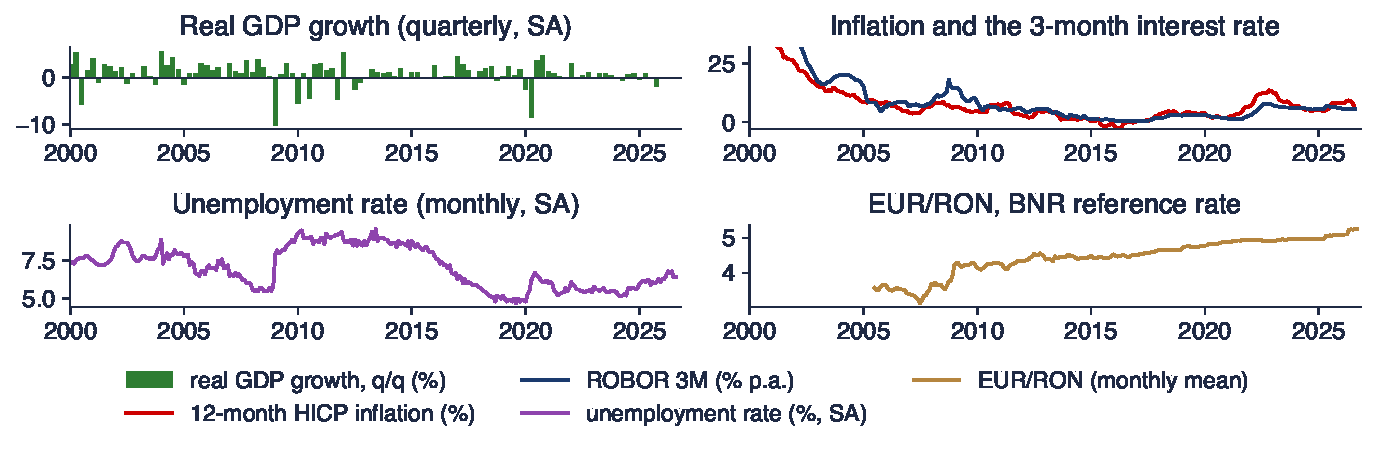
\includegraphics[width=0.97\textwidth,height=0.6\textheight,keepaspectratio]{tsa_ch6_ro_macro.pdf}
\end{center}
\vspace{-0.25cm}
\begin{itemize}
    \item Creșterea PIB-ului real (Eurostat, față de trimestrul anterior, ajustat sezonier); inflația anuală IAPC (Eurostat); ROBOR 3M, dobînda interbancară la 3 luni (Eurostat); rata șomajului (Eurostat, ajustată sezonier); EUR/RON, cursul de referință BNR
\end{itemize}
\quantlet{TSA\_ch6\_multivariate\_data}{\qlurl{TSA_ch6_multivariate_data}}
\end{frame}

\begin{frame}{Interpretarea seriilor românești}
\itemsize{\small}
\begin{itemize}
    \item Inflația și ROBOR 3M cresc și scad împreună: corelația este 0{,}66 în T1 2005--T2 2026 (medii trimestriale)
    \begin{itemize}
        \item inflația a atins 13{,}6\% în noiembrie 2022; ROBOR 3M a atins 18{,}2\% în octombrie 2008 (criza de lichiditate din 2008)
    \end{itemize}
    \item Creșterea PIB-ului este zgomotoasă, cu două scăderi mari: -10{,}2\% în T1 2009 și -8{,}6\% în T2 2020
    \begin{itemize}
        \item ultimele valori: inflația 6{,}1\% (august 2026), ROBOR 3M 5{,}69\%, șomajul 6{,}4\%, EUR/RON 5{,}26
    \end{itemize}
    \item Întrebările capitolului
    \begin{itemize}
        \item Ajută inflația la prognoza dobînzii?
        \item Cum reacționează ROBOR la o surpriză a inflației și cît timp?
    \end{itemize}
\end{itemize}
\end{frame}

\begin{frame}{Serii de timp vectoriale}
\itemsize{\small}
\begin{itemize}
    \item \textbf{Definiție}: $\bY_t = (Y_{1t}, \dots, Y_{Kt})'$ grupează $K$ serii observate la aceleași date
    \begin{itemize}
        \item exemplu: $\bY_t = (g_t, \pi_t, i_t)'$, creșterea PIB-ului, inflația și ROBOR 3M din trimestrul $t$; $K = 3$
    \end{itemize}
    \item \textbf{Vectorul mediilor}: $\boldsymbol{\mu} = E[\bY_t]$, de dimensiune $K \times 1$
    \begin{itemize}
        \item \textbf{matricea de autocovarianță} la decalajul $h$: $\bGamma(h) = \Cov(\bY_t, \bY_{t-h}) = E[(\bY_t - \boldsymbol{\mu})(\bY_{t-h} - \boldsymbol{\mu})']$, $K \times K$
        \item diagonala: autocovarianțele fiecărei serii (\tsachlink{https://danpele.github.io/Time-Series-Analysis/RO/Cursuri/capitol1_procese_stochastice_stationaritate.pdf}{Capitolul 1}); în afara diagonalei: \textbf{covarianțele încrucișate} $\gamma_{jk}(h) = \Cov(Y_{jt}, Y_{k,t-h})$
    \end{itemize}
    \item \textbf{Staționaritate slabă}: $\boldsymbol{\mu}$ și $\bGamma(h)$ nu depind de $t$
    \begin{itemize}
        \item $\bGamma(h)$ nu este simetrică, dar $\bGamma(-h) = \bGamma(h)'$: „$Y_1$ precedă $Y_2$” și „$Y_2$ precedă $Y_1$” sînt afirmații diferite
    \end{itemize}
\end{itemize}
\end{frame}

\begin{frame}{Funcția de corelație încrucișată}
\itemsize{\small}
\begin{itemize}
    \item \textbf{Definiție}: $\rho_{yx}(k) = \Corr(y_t, x_{t-k}) = \gamma_{yx}(k)/(\sigma_y\sigma_x)$, pentru $k = 0, \pm 1, \pm 2, \dots$
    \begin{itemize}
        \item funcția de corelație încrucișată (CCF): $k > 0$: $x$ din trecut cu $y$ de azi ($x$ precedă); $k < 0$: $y$ precedă
    \end{itemize}
    \item Versiunea de eșantion: $\hat\rho_{yx}(k)$, corelația perechilor $(y_t, x_{t-k})$
    \begin{itemize}
        \item dacă cele două serii sînt zgomote albe independente, $\hat\rho_{yx}(k) \approx N(0, 1/T)$: benzile $\pm 1{,}96/\sqrt{T}$
        \item pentru serii autocorelate benzile sînt prea înguste: apar relații false de precedență (comparați cu \tsachlink{https://danpele.github.io/Time-Series-Analysis/RO/Cursuri/capitol3_radacini_unitare_modele_arima.pdf}{Capitolul 3}, regresia falsă)
    \end{itemize}
    \item CCF privește o pereche și un decalaj pe rînd; un VAR privește împreună toate variabilele și toate decalajele
\end{itemize}
\end{frame}

\begin{frame}{Corelații încrucișate: piețe și date macroeconomice românești}
\itemsize{\footnotesize}
\begin{center}
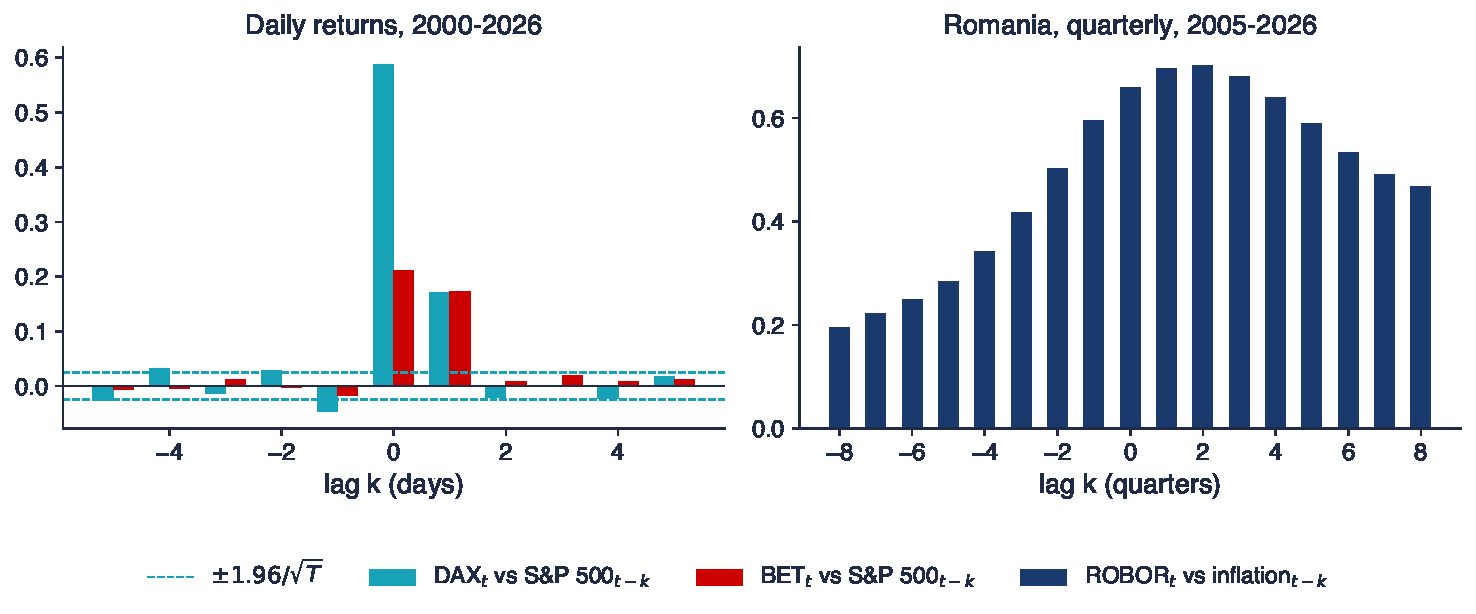
\includegraphics[width=0.97\textwidth,height=0.56\textheight,keepaspectratio]{tsa_ch6_ccf.pdf}
\end{center}
\vspace{-0.25cm}
\begin{itemize}
    \item Stînga: randamente logaritmice zilnice (EODHD), 6\,433 de zile comune de tranzacționare, 2000--2026; bare: $\Corr(\text{DAX}_t, \text{S\&P}_{t-k})$ și $\Corr(\text{BET}_t, \text{S\&P}_{t-k})$. Dreapta: ROBOR 3M trimestrial față de decalajele inflației
\end{itemize}
\quantlet{TSA\_ch6\_multivariate\_data}{\qlurl{TSA_ch6_multivariate_data}}
\end{frame}

\begin{frame}{Interpretarea corelațiilor încrucișate}
\itemsize{\small}
\begin{itemize}
    \item BET cu S\&P 500: 0{,}21 în aceeași zi și 0{,}17 cu ziua precedentă ($k = 1$); pentru $k = -1$: -0{,}02
    \begin{itemize}
        \item banda este $\pm$0{,}024: randamentul de ieri de la New York se vede în randamentele de azi de la București și Frankfurt, nu invers
        \item motivul: Wall Street se închide la ora 22:00 (ora Frankfurtului), după piețele europene; știrile ajung la ele a doua zi dimineață
    \end{itemize}
    \item ROBOR cu inflația: cea mai mare corelație, 0{,}70, apare la $k = 2$ trimestre (inflația precedă)
    \begin{itemize}
        \item dar toate valorile sînt mari (0{,}34 la $k = -4$, 0{,}64 la $k = 4$): două serii persistente; CCF singură nu poate separa precedența de persistență
    \end{itemize}
\end{itemize}
\end{frame}

\begin{frame}{De ce un singur model pentru toate seriile}
\itemsize{\small}
\begin{itemize}
    \item Modelele univariate (\tsachlink{https://danpele.github.io/Time-Series-Analysis/RO/Cursuri/capitol2_modele_arma.pdf}{Capitolele 2}--\tsachlink{https://danpele.github.io/Time-Series-Analysis/RO/Cursuri/capitol3_radacini_unitare_modele_arima.pdf}{3}) prognozează fiecare serie din propriul trecut
    \begin{itemize}
        \item ele ignoră faptul că inflația din trimestrul trecut poate ajuta la prognoza dobînzii din acest trimestru
    \end{itemize}
    \item \textbf{Feedback}: banca centrală reacționează la inflație, inflația reacționează la dobîndă
    \begin{itemize}
        \item o singură regresie a lui $\pi_t$ pe $i_t$ tratează $i_t$ ca fiind dat (exogen); aici ambele sînt \textbf{endogene}, determinate în interiorul sistemului
    \end{itemize}
    \item Un VAR tratează simetric toate variabilele: fiecare depinde de trecutul tuturor
    \begin{itemize}
        \item nu este nevoie de teorie economică pentru a-l scrie; teoria revine cînd interpretăm șocurile (secțiunea 7)
    \end{itemize}
\end{itemize}
\end{frame}

\begin{frame}{Recapitulare: de la o serie la mai multe}
\itemsize{\small}
\begin{itemize}
    \item O serie vectorială $\bY_t$ are un vector al mediilor și matrice de autocovarianță $\bGamma(h)$, cu $\bGamma(-h) = \bGamma(h)'$
    \item CCF $\rho_{yx}(k)$ arată relațiile de precedență; $k > 0$: $x$ precedă
    \item Randamentele S\&P 500 precedă cu o zi randamentele DAX și BET
    \item Feedback-ul dintre variabile cere un model comun
\end{itemize}
\end{frame}


%=============================================================================
\section{Modelul VAR$(p)$}
%=============================================================================

\begin{frame}{Modelul VAR$(p)$}
\itemsize{\small}
\begin{itemize}
    \item \textbf{Definiție}: $\bY_t = \bc + \bA_1\bY_{t-1} + \dots + \bA_p\bY_{t-p} + \bepsilon_t$
    \begin{itemize}
        \item $\bc$: vectorul termenilor liberi, $K \times 1$; $\bA_1, \dots, \bA_p$: matricele coeficienților, $K \times K$
        \item $\bepsilon_t$: zgomot alb vectorial: $E[\bepsilon_t] = \mathbf{0}$, $E[\bepsilon_t\bepsilon_t'] = \bSigma$, $E[\bepsilon_t\bepsilon_s'] = \mathbf{0}$ pentru $t \ne s$
    \end{itemize}
    \item $\bSigma$ nu este, în general, diagonală: șocurile din ecuații diferite sînt corelate \textbf{la aceeași dată}
    \begin{itemize}
        \item erorile de la date diferite nu sînt corelate: toată dinamica se află în matricele $\bA_j$
    \end{itemize}
    \item Pentru $K = 1$ regăsim modelul AR$(p)$ din \tsachlink{https://danpele.github.io/Time-Series-Analysis/RO/Cursuri/capitol2_modele_arma.pdf}{Capitolul 2}
    \begin{itemize}
        \item această formă se numește \textbf{forma redusă}: descrie datele, nu șocurile economice (secțiunea 10)
    \end{itemize}
\end{itemize}
\end{frame}

\begin{frame}{Un VAR(1) cu două variabile, ecuație cu ecuație}
\itemsize{\small}
\begin{itemize}
    \item În formă matriceală:
    \begin{itemize}
        \item $\begin{pmatrix} y_{1t} \\ y_{2t} \end{pmatrix} = \begin{pmatrix} c_1 \\ c_2 \end{pmatrix} + \begin{pmatrix} a_{11} & a_{12} \\ a_{21} & a_{22} \end{pmatrix}\begin{pmatrix} y_{1,t-1} \\ y_{2,t-1} \end{pmatrix} + \begin{pmatrix} \varepsilon_{1t} \\ \varepsilon_{2t} \end{pmatrix}$
    \end{itemize}
    \item Ecuație cu ecuație:
    \begin{itemize}
        \item $y_{1t} = c_1 + a_{11}y_{1,t-1} + a_{12}y_{2,t-1} + \varepsilon_{1t}$
        \item $y_{2t} = c_2 + a_{21}y_{1,t-1} + a_{22}y_{2,t-1} + \varepsilon_{2t}$
    \end{itemize}
    \item Interpretarea coeficienților: $a_{jk}$ = efectul lui $y_{k,t-1}$ asupra lui $y_{jt}$ (rîndul: ecuația; coloana: regresorul)
    \begin{itemize}
        \item $a_{12} = a_{21} = 0$: două modele AR(1) separate; $a_{12} \ne 0$: trecutul lui $y_2$ ajută la prognoza lui $y_1$
    \end{itemize}
\end{itemize}
\end{frame}

\begin{frame}{Exemplu rezolvat: un VAR(1)}
\itemsize{\small}
\begin{itemize}
    \item Modelul: $\bc = (1{,}2;\ 0{,}6)'$, $\bA = \begin{pmatrix} 0{,}5 & 0{,}2 \\ 0{,}3 & 0{,}4 \end{pmatrix}$, $\bSigma = \begin{pmatrix} 1 & 0{,}5 \\ 0{,}5 & 1 \end{pmatrix}$
    \begin{itemize}
        \item $y_{1t} = 1{,}2 + 0{,}5y_{1,t-1} + 0{,}2y_{2,t-1} + \varepsilon_{1t}$; \quad $y_{2t} = 0{,}6 + 0{,}3y_{1,t-1} + 0{,}4y_{2,t-1} + \varepsilon_{2t}$
    \end{itemize}
    \item Interpretare: $a_{21} = 0{,}3$: o unitate în plus a lui $y_1$ în perioada trecută crește $y_2$ cu 0,3 azi, celelalte fiind fixe
    \begin{itemize}
        \item șocurile sînt corelate: $\Corr(\varepsilon_{1t}, \varepsilon_{2t}) = 0{,}5$
    \end{itemize}
    \item Prognoze din $\bY_T = (5;\ 2)'$: $\hat\bY_{T+1} = \bc + \bA\bY_T = \begin{pmatrix} 4{,}10 \\ 2{,}90 \end{pmatrix}$, \quad $\hat\bY_{T+2} = \bc + \bA\hat\bY_{T+1} = \begin{pmatrix} 3{,}83 \\ 2{,}99 \end{pmatrix}$
    \begin{itemize}
        \item prognozele se îndreaptă spre medie, $\boldsymbol{\mu} = (3{,}50; 2{,}75)'$ (secțiunea următoare)
    \end{itemize}
\end{itemize}
\end{frame}

\begin{frame}{Exemplul rezolvat, simulat}
\itemsize{\footnotesize}
\begin{center}
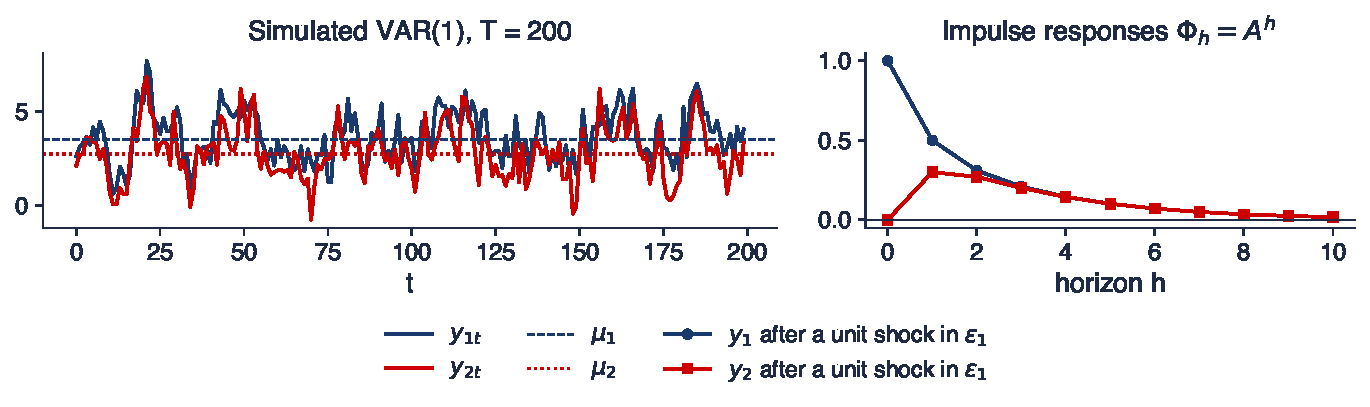
\includegraphics[width=0.97\textwidth,height=0.56\textheight,keepaspectratio]{tsa_ch6_var_sim.pdf}
\end{center}
\vspace{-0.25cm}
\begin{itemize}
    \item Stînga: 200 de perioade din modelul VAR(1) de pe slide-ul anterior, cu cele două medii; dreapta: răspunsurile lui $y_1$ și $y_2$ la un șoc unitar în $\varepsilon_1$ la $h = 0$, coloanele lui $\bA^h$
\end{itemize}
\quantlet{TSA\_ch6\_var\_stability}{\qlurl{TSA_ch6_var_stability}}
\end{frame}

\begin{frame}{Interpretarea VAR(1) simulat}
\itemsize{\small}
\begin{itemize}
    \item Cele două serii oscilează în jurul mediilor și evoluează împreună: corelația de eșantion este 0{,}75
    \begin{itemize}
        \item două surse ale evoluției comune: șocurile corelate ($\Corr = 0{,}5$) și efectele încrucișate $a_{12}$, $a_{21}$
    \end{itemize}
    \item Un șoc unitar în $y_1$ ajunge la $y_2$ după o perioadă ($a_{21} = 0{,}3$), apoi ambele se sting
    \begin{itemize}
        \item stingerea este guvernată de cea mai mare valoare proprie a lui $\bA$, 0{,}7: după 5 perioade rămîne circa $0{,}7^5 \approx 0{,}17$ din efect
    \end{itemize}
\end{itemize}
\end{frame}

\begin{frame}{Cîți parametri?}
\itemsize{\small}
\begin{itemize}
    \item Un VAR$(p)$ cu $K$ variabile și termen liber: $K + pK^2$ coeficienți, plus $K(K+1)/2$ în $\bSigma$
    \begin{itemize}
        \item fiecare ecuație are $1 + pK$ regresori
        \item VAR-ul românesc: $K = 3$, $p = 2$: $3 + 2 \cdot 9 = 21$ coeficienți estimați pe 84 trimestre
    \end{itemize}
    \item \textbf{Blestemul dimensionalității}: $K = 5$, $p = 4$: $5 + 4 \cdot 25 = 105$ de coeficienți
    \begin{itemize}
        \item cu 25 de ani de date trimestriale (100 de observații) fiecare ecuație are 21 de regresori și 79 de grade de libertate reziduale
    \end{itemize}
    \item De aici VAR-uri mici (3--6 variabile), puține decalaje și estimări cu erori standard mari; coeficienții individuali se interpretează rar
\end{itemize}
\end{frame}

\begin{frame}{Christopher Sims și „Macroeconomics and Reality”}
\itemsize{\small}
\begin{columns}[T]
\begin{column}{0.38\textwidth}
\centering

\includegraphics[height=0.56\textheight]{ch6_christopher_sims_2011.jpg}\\[1mm]
\imgcap{Christopher A. Sims, Premiul Nobel pentru economie 2011}
\imgcredit{https://commons.wikimedia.org/wiki/File:Christopher_A._Sims_close-up_(cropped).jpg}{Foto: Holger Motzkau (2011); CC BY-SA 3.0; Wikimedia Commons}
\end{column}
\begin{column}{0.6\textwidth}
\begin{itemize}
    \item \refSims: marile modele macroeconomice din anii 1970 impuneau restricții „incredibile” (ce variabile sînt exogene, ce decalaje sînt nule)
    \begin{itemize}
        \item propunerea lui: lăsăm datele să vorbească printr-un VAR nerestricționat, apoi adăugăm doar puținele ipoteze necesare pentru interpretarea șocurilor
    \end{itemize}
    \item VAR-ul a devenit instrumentul standard al băncilor centrale pentru prognoză și pentru măsurarea efectelor politicii monetare
    \item Premiul Nobel 2011, împreună cu Thomas Sargent, „pentru cercetarea empirică a cauzei și efectului în macroeconomie”
\end{itemize}
\end{column}
\end{columns}
\end{frame}

\begin{frame}{Recapitulare: modelul VAR$(p)$}
\itemsize{\small}
\begin{itemize}
    \item $\bY_t = \bc + \sum_{j=1}^{p}\bA_j\bY_{t-j} + \bepsilon_t$, $\bepsilon_t$ zgomot alb cu covarianța $\bSigma$
    \item $a_{jk}$: efectul decalajului variabilei $k$ în ecuația variabilei $j$
    \item $K + pK^2$ coeficienți: păstrăm $K$ și $p$ mici
    \item \refSims: VAR-ul ca alternativă la restricțiile „incredibile”
\end{itemize}
\end{frame}


%=============================================================================
\section{Staționaritate și forma companion}
%=============================================================================

\begin{frame}{Stabilitatea unui VAR(1)}
\itemsize{\small}
\begin{itemize}
    \item Substituim repetat: $\bY_t = \bc + \bA\bc + \dots + \bA^{h-1}\bc + \bA^h\bY_{t-h} + \sum_{j=0}^{h-1}\bA^j\bepsilon_{t-j}$
    \begin{itemize}
        \item trecutul este uitat doar dacă $\bA^h \to \mathbf{0}$
    \end{itemize}
    \item \textbf{Condiția de stabilitate}: toate valorile proprii $\lambda$ ale lui $\bA$ au $|\lambda| < 1$
    \begin{itemize}
        \item valorile proprii: rădăcinile ecuației $\det(\bA - \lambda\mathbf{I}) = 0$; pentru $K = 2$: $\lambda^2 - \mathrm{tr}(\bA)\lambda + \det(\bA) = 0$
        \item un VAR stabil este slab staționar (dacă a pornit demult); aceasta este versiunea multivariată a condiției $|\phi| < 1$ (\tsachlink{https://danpele.github.io/Time-Series-Analysis/RO/Cursuri/capitol2_modele_arma.pdf}{Capitolul 2})
    \end{itemize}
    \item \textbf{Exemplu}: $\mathrm{tr}(\bA) = 0{,}9$, $\det(\bA) = 0{,}5 \cdot 0{,}4 - 0{,}2 \cdot 0{,}3 = 0{,}14$: $\lambda^2 - 0{,}9\lambda + 0{,}14 = 0$
    \begin{itemize}
        \item $\lambda = (0{,}9 \pm 0{,}5)/2$: $\lambda_1 = 0{,}7$, $\lambda_2 = 0{,}2$; ambele în interiorul cercului unitate: stabil
    \end{itemize}
\end{itemize}
\end{frame}

\begin{frame}{Media și varianța unui VAR(1) stabil}
\itemsize{\small}
\begin{itemize}
    \item \textbf{Media}: aplicăm media, $\boldsymbol{\mu} = \bc + \bA\boldsymbol{\mu}$, deci $\boldsymbol{\mu} = (\mathbf{I} - \bA)^{-1}\bc$
    \begin{itemize}
        \item exemplu: $\mathbf{I} - \bA = \begin{pmatrix} 0{,}5 & -0{,}2 \\ -0{,}3 & 0{,}6 \end{pmatrix}$, determinantul 0{,}24; $\boldsymbol{\mu} = \frac{1}{0{,}24}\begin{pmatrix} 0{,}6 & 0{,}2 \\ 0{,}3 & 0{,}5 \end{pmatrix}\begin{pmatrix} 1{,}2 \\ 0{,}6 \end{pmatrix} = \begin{pmatrix} 3{,}50 \\ 2{,}75 \end{pmatrix}$
    \end{itemize}
    \item \textbf{Varianța}: $\bGamma(0) = \bA\bGamma(0)\bA' + \bSigma$ (o ecuație Lyapunov discretă); $\bGamma(h) = \bA^h\bGamma(0)$
    \begin{itemize}
        \item se rezolvă prin $\mathrm{vec}\,\bGamma(0) = (\mathbf{I} - \bA \otimes \bA)^{-1}\mathrm{vec}\,\bSigma$; exemplu: $\bGamma(0) = \begin{pmatrix} 1{,}75 & 1{,}22 \\ 1{,}22 & 1{,}73 \end{pmatrix}$
        \item $\otimes$: produsul Kronecker; $\mathrm{vec}$ așază coloanele unei matrice una sub alta
    \end{itemize}
    \item Varianțele 1{,}75 și 1{,}73 depășesc varianța șocurilor (1): dinamica acumulează șocurile trecute
\end{itemize}
\end{frame}

\begin{frame}{Forma companion a unui VAR$(p)$}
\itemsize{\small}
\begin{itemize}
    \item Grupăm $p$ vectori consecutivi: $\boldsymbol{\xi}_t = (\bY_t', \bY_{t-1}', \dots, \bY_{t-p+1}')'$, de dimensiune $Kp$
    \begin{itemize}
        \item atunci $\boldsymbol{\xi}_t = \boldsymbol{\nu} + \mathbf{F}\boldsymbol{\xi}_{t-1} + \mathbf{v}_t$: orice VAR$(p)$ este un VAR(1) în $\boldsymbol{\xi}_t$
    \end{itemize}
    \item Pentru $p = 2$: $\begin{pmatrix} \bY_t \\ \bY_{t-1} \end{pmatrix} = \begin{pmatrix} \bc \\ \mathbf{0} \end{pmatrix} + \underbrace{\begin{pmatrix} \bA_1 & \bA_2 \\ \mathbf{I}_K & \mathbf{0} \end{pmatrix}}_{\mathbf{F}}\begin{pmatrix} \bY_{t-1} \\ \bY_{t-2} \end{pmatrix} + \begin{pmatrix} \bepsilon_t \\ \mathbf{0} \end{pmatrix}$
    \begin{itemize}
        \item al doilea bloc de rînduri este identitatea $\bY_{t-1} = \bY_{t-1}$
    \end{itemize}
    \item \textbf{Stabilitatea unui VAR$(p)$}: toate cele $Kp$ valori proprii ale matricei companion $\mathbf{F}$ au modulul sub 1
    \begin{itemize}
        \item echivalent: toate rădăcinile ecuației $\det(\mathbf{I}_K - \bA_1z - \dots - \bA_pz^p) = 0$ sînt în afara cercului unitate
        \item valorile proprii ale lui $\bA_1$ singure nu spun nimic despre stabilitatea unui VAR(2)
    \end{itemize}
\end{itemize}
\end{frame}

\begin{frame}{Valorile proprii a trei VAR-uri estimate}
\itemsize{\footnotesize}
\begin{center}
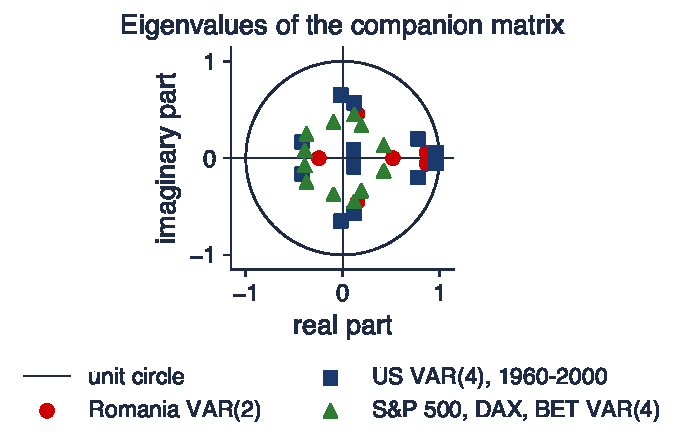
\includegraphics[width=0.97\textwidth,height=0.6\textheight,keepaspectratio]{tsa_ch6_roots.pdf}
\end{center}
\vspace{-0.25cm}
\begin{itemize}
    \item Matricele companion: VAR(2) românesc (creșterea PIB-ului, inflația, ROBOR 3M; 6 valori proprii), VAR(4) american din secțiunea 10 (12), VAR(4) zilnic pentru S\&P 500, DAX și BET (12)
\end{itemize}
\quantlet{TSA\_ch6\_var\_stability}{\qlurl{TSA_ch6_var_stability}}
\end{frame}

\begin{frame}{Interpretarea valorilor proprii}
\itemsize{\small}
\begin{itemize}
    \item Toate cele trei VAR-uri sînt stabile; cele mai mari module: România 0{,}869, SUA 0{,}969, piețe 0{,}464
    \begin{itemize}
        \item cel mai mare modul stabilește viteza cu care se sting șocurile: $0{,}97^{20} \approx 0{,}54$ după 20 de trimestre, $0{,}46^{2} \approx 0{,}21$ după 2 zile
    \end{itemize}
    \item VAR-urile macroeconomice au valori proprii apropiate de 1 (inflație și dobînzi persistente); VAR-urile de randamente au valori mici
    \begin{itemize}
        \item perechile complexe produc oscilații amortizate în răspunsuri
    \end{itemize}
    \item O valoare proprie foarte apropiată de 1 semnalează o rădăcină unitară, poate cointegrare: Capitolul 7
\end{itemize}
\end{frame}

\begin{frame}{Reprezentarea de medie mobilă}
\itemsize{\small}
\begin{itemize}
    \item Un VAR stabil se poate scrie ca o medie mobilă infinită a șocurilor (Wold, \tsachlink{https://danpele.github.io/Time-Series-Analysis/RO/Cursuri/capitol1_procese_stochastice_stationaritate.pdf}{Capitolul 1}):
    \begin{itemize}
        \item $\bY_t = \boldsymbol{\mu} + \bepsilon_t + \bPhi_1\bepsilon_{t-1} + \bPhi_2\bepsilon_{t-2} + \dots = \boldsymbol{\mu} + \sum_{h=0}^{\infty}\bPhi_h\bepsilon_{t-h}$, $\bPhi_0 = \mathbf{I}$
    \end{itemize}
    \item VAR(1): $\bPhi_h = \bA^h$; VAR$(p)$: $\bPhi_h = \sum_{j=1}^{\min(h,p)}\bA_j\bPhi_{h-j}$
    \begin{itemize}
        \item exemplu: $\bPhi_2 = \bA^2 = \begin{pmatrix} 0{,}31 & 0{,}18 \\ 0{,}27 & 0{,}22 \end{pmatrix}$
    \end{itemize}
    \item Elementul $(j, k)$ al lui $\bPhi_h$: efectul asupra lui $Y_{j,t+h}$ al unei modificări unitare a lui $\varepsilon_{kt}$, celelalte șocuri fiind fixe
    \begin{itemize}
        \item acestea sînt \textbf{răspunsurile la impuls} (secțiunea 7); tot din ele obținem erorile de prognoză (secțiunile 8--9)
    \end{itemize}
\end{itemize}
\end{frame}

\begin{frame}{Recapitulare: staționaritate și forma companion}
\itemsize{\small}
\begin{itemize}
    \item VAR(1): stabil dacă toate valorile proprii ale lui $\bA$ au $|\lambda| < 1$; VAR$(p)$: aceeași condiție pentru matricea companion
    \item Media $\boldsymbol{\mu} = (\mathbf{I} - \bA_1 - \dots - \bA_p)^{-1}\bc$; prognozele converg spre ea
    \item Forma de medie mobilă $\bY_t = \boldsymbol{\mu} + \sum_h\bPhi_h\bepsilon_{t-h}$: baza răspunsurilor la impuls
    \item VAR-urile macroeconomice estimate au valori proprii apropiate de 1
\end{itemize}
\end{frame}


%=============================================================================
\section{Estimare și alegerea numărului de decalaje}
%=============================================================================

\begin{frame}{Estimarea prin OLS, ecuație cu ecuație}
\itemsize{\small}
\begin{itemize}
    \item Fiecare ecuație este o regresie liniară a lui $Y_{jt}$ pe o constantă și pe $\bY_{t-1}, \dots, \bY_{t-p}$
    \begin{itemize}
        \item aceiași $1 + Kp$ regresori în fiecare ecuație; OLS (ordinary least squares, metoda celor mai mici pătrate) pe fiecare ecuație separat
    \end{itemize}
    \item \textbf{De ce ajunge OLS}: cu regresori identici, estimarea sistemului (GLS pe toate ecuațiile) dă exact estimările OLS
    \begin{itemize}
        \item corelația șocurilor nu îmbunătățește estimările; cu erori Normale, OLS este și estimatorul de verosimilitate maximă
    \end{itemize}
    \item \textbf{Covarianța șocurilor}: $\hat\bSigma = \frac{1}{T - Kp - 1}\sum_t\hat\bepsilon_t\hat\bepsilon_t'$, din reziduurile tuturor ecuațiilor
    \begin{itemize}
        \item staționaritatea contează: pentru serii staționare testele $t$ și $F$ obișnuite sînt valide în eșantioane mari
    \end{itemize}
\end{itemize}
\end{frame}

\begin{frame}{Alegerea lui $p$: criterii informaționale}
\itemsize{\small}
\begin{itemize}
    \item Estimăm VAR$(p)$ pentru $p = 0, \dots, p_{\max}$ pe \textbf{același eșantion}; $\tilde\bSigma(p)$: covarianța reziduurilor împărțită la $T$
    \begin{itemize}
        \item AIC (Akaike) $= \ln\det\tilde\bSigma(p) + \frac{2}{T}pK^2$ \refAkaike
        \item BIC (Schwarz) $= \ln\det\tilde\bSigma(p) + \frac{\ln T}{T}pK^2$ \refSchwarz
        \item HQ (Hannan--Quinn) $= \ln\det\tilde\bSigma(p) + \frac{2\ln\ln T}{T}pK^2$ \refHQ
    \end{itemize}
    \item Primul termen: calitatea ajustării („volumul” reziduurilor mai mic); al doilea: o penalizare pe coeficient; alegem $p$ cu cea mai mică valoare
    \begin{itemize}
        \item penalizările: AIC $<$ HQ $<$ BIC (pentru $T \ge 16$): BIC alege cel mai mic $p$, AIC cel mai mare
        \item BIC și HQ sînt consistente (găsesc $p$ adevărat cînd $T \to \infty$); AIC tinde să supraajusteze, dar prognozează adesea bine
    \end{itemize}
\end{itemize}
\end{frame}

\begin{frame}{VAR-ul românesc: ce $p$?}
\itemsize{\footnotesize}
\begin{center}
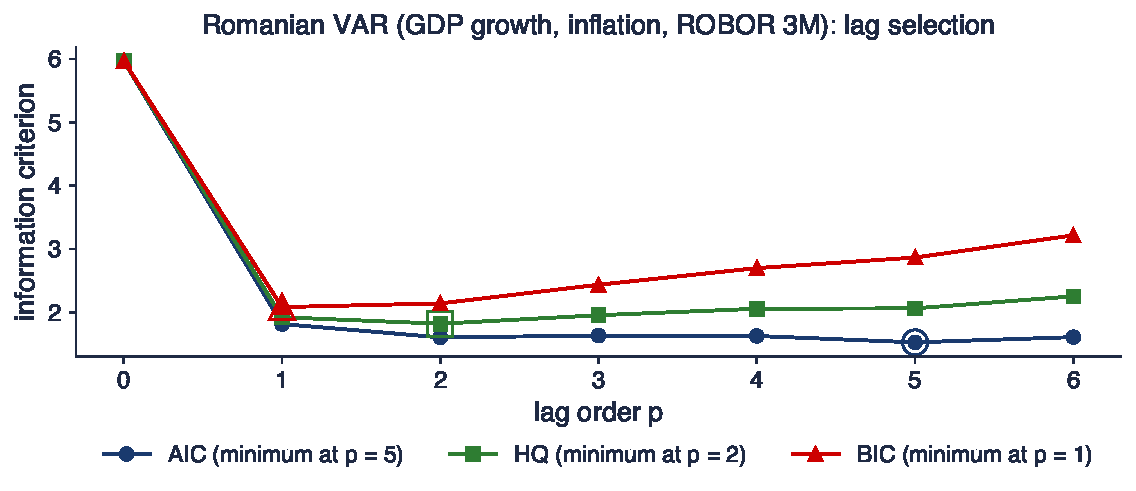
\includegraphics[width=0.97\textwidth,height=0.56\textheight,keepaspectratio]{tsa_ch6_ic.pdf}
\end{center}
\vspace{-0.25cm}
\begin{itemize}
    \item Creșterea PIB-ului, inflația anuală și ROBOR 3M, T1 2005--T2 2026; VAR$(p)$ pentru $p = 0, \dots, 6$ pe eșantionul comun de 80 de trimestre; cercurile marchează minimele
\end{itemize}
\quantlet{TSA\_ch6\_estimation\_diagnostics}{\qlurl{TSA_ch6_estimation_diagnostics}}
\end{frame}

\begin{frame}{Interpretarea alegerii numărului de decalaje}
\itemsize{\small}
\begin{itemize}
    \item BIC alege $p = 1$, HQ $p = 2$, AIC $p = 5$: cele trei criterii nu coincid, cum se întîmplă adesea în eșantioane scurte
    \begin{itemize}
        \item AIC: 1{,}812 pentru $p = 1$, 1{,}603 pentru $p = 2$, 1{,}523 pentru $p = 5$: o curbă plată după $p = 2$
    \end{itemize}
    \item $p = 5$ ar însemna $3 + 5 \cdot 9 = 48$ de coeficienți pentru circa 80 de trimestre
    \begin{itemize}
        \item alegem $p = 2$ (HQ), apoi verificăm dacă reziduurile sînt zgomot alb; dacă nu, adăugăm decalaje
    \end{itemize}
    \item O regulă practică: pornim de la criterii, dar nu ne oprim la ele
\end{itemize}
\end{frame}

\begin{frame}{VAR(2) românesc estimat}
\itemsize{\small}
\begin{center}
\scriptsize
\begin{tabular}{lrrr}
\toprule
\textbf{Regresorul} & \textbf{ecuația $g_t$} & \textbf{ecuația $\pi_t$} & \textbf{ecuația $i_t$} \\
\midrule
termen liber & $1{,}09$ ($2{,}1$) & $0{,}49$ ($2{,}0$) & $-0{,}11$ ($-0{,}6$) \\
$g_{t-1}$ & $0{,}01$ ($0{,}1$) & $0{,}01$ ($0{,}1$) & $0{,}14$ ($3{,}5$) \\
$\pi_{t-1}$ & $0{,}53$ ($2{,}3$) & $1{,}26$ ($11{,}7$) & $0{,}24$ ($2{,}8$) \\
$i_{t-1}$ & $-0{,}73$ ($-2{,}7$) & $0{,}16$ ($1{,}2$) & $1{,}04$ ($10{,}2$) \\
$g_{t-2}$ & $-0{,}08$ ($-0{,}7$) & $-0{,}03$ ($-0{,}5$) & $0{,}07$ ($1{,}7$) \\
$\pi_{t-2}$ & $-0{,}41$ ($-1{,}7$) & $-0{,}35$ ($-3{,}1$) & $-0{,}17$ ($-1{,}9$) \\
$i_{t-2}$ & $0{,}54$ ($2{,}0$) & $-0{,}16$ ($-1{,}3$) & $-0{,}12$ ($-1{,}2$) \\
$R^2$ & 0{,}16 & 0{,}90 & 0{,}93 \\
\bottomrule
\end{tabular}
\end{center}
\begin{itemize}
    \item OLS pe 84 de trimestre (T3 2005--T2 2026); statisticile $t$ între paranteze; 21 de coeficienți
    \item Abaterile standard ale reziduurilor: 2{,}32 ($g$), 1{,}09 ($\pi$), 0{,}87 ($i$); corelația reziduurilor lui $\pi$ și $i$: 0{,}25
\end{itemize}
\end{frame}

\begin{frame}{Interpretarea coeficienților}
\itemsize{\small}
\begin{itemize}
    \item Inflația este foarte persistentă: $1{,}26\,\pi_{t-1} -0{,}35\,\pi_{t-2}$; la fel ROBOR: $1{,}04\,i_{t-1}$
    \begin{itemize}
        \item $R^2$ de 0{,}90 și 0{,}93: cea mai mare parte provine din propriul trecut al seriilor
    \end{itemize}
    \item În ecuația ROBOR contează creșterea PIB-ului din trecut ($t = 3{,}5$) și inflația din trecut ($t = 2{,}8$): dobînda urmează economia
    \begin{itemize}
        \item Creșterea PIB-ului este greu de prognozat: $R^2 = 0{,}16$
    \end{itemize}
    \item Coeficienții individuali ai unor decalaje corelate sînt instabili (de exemplu $i_{t-1}$ și $i_{t-2}$ cu semne opuse în ecuația lui $g$): interpretăm sistemul prin teste, răspunsuri și prognoze, nu coeficient cu coeficient
\end{itemize}
\end{frame}

\begin{frame}{Recapitulare: estimare și alegerea numărului de decalaje}
\itemsize{\small}
\begin{itemize}
    \item OLS ecuație cu ecuație este eficient: toate ecuațiile au aceiași regresori
    \item AIC, BIC, HQ: $\ln\det\tilde\bSigma(p)$ plus o penalizare; comparăm pe un eșantion comun
    \item BIC $\le$ HQ $\le$ AIC ca $p$ ales; VAR-ul românesc: $p = 2$
    \item Interpretăm sistemul, nu coeficienții individuali
\end{itemize}
\end{frame}


%=============================================================================
\section{Diagnosticarea reziduurilor}
%=============================================================================

\begin{frame}{Sînt reziduurile zgomot alb?}
\itemsize{\small}
\begin{itemize}
    \item \textbf{Testul portmanteau multivariat} \refHosking: $H_0$: nicio autocorelație și nicio corelație încrucișată a reziduurilor pînă la decalajul $h$
    \begin{itemize}
        \item $Q_h = T^2\sum_{j=1}^{h}\frac{1}{T - j}\mathrm{tr}(\hat{\mathbf{C}}_j'\hat{\mathbf{C}}_0^{-1}\hat{\mathbf{C}}_j\hat{\mathbf{C}}_0^{-1})$, $\hat{\mathbf{C}}_j$: matricele de autocovarianță ale reziduurilor
        \item în ipoteza $H_0$: $\chi^2$ cu $K^2(h - p)$ grade de libertate; testul Ljung--Box multivariat (\tsachlink{https://danpele.github.io/Time-Series-Analysis/RO/Cursuri/capitol2_modele_arma.pdf}{Capitolul 2})
    \end{itemize}
    \item \textbf{Normalitatea}: un test Jarque--Bera multivariat \refJB\ pe reziduurile standardizate (asimetrie și boltire)
    \begin{itemize}
        \item normalitatea nu este necesară pentru OLS; contează pentru intervale exacte și pentru eșantioane mici
    \end{itemize}
    \item Dacă testul portmanteau respinge: adăugăm decalaje, adăugăm o variabilă sau modelăm rupturile și valorile extreme (variabile dummy)
    \begin{itemize}
        \item verificăm și stabilitatea (valorile proprii) și, pentru eșantioane lungi, stabilitatea parametrilor în timp
    \end{itemize}
\end{itemize}
\end{frame}

\begin{frame}{Reziduurile VAR(2) românesc}
\itemsize{\footnotesize}
\begin{center}
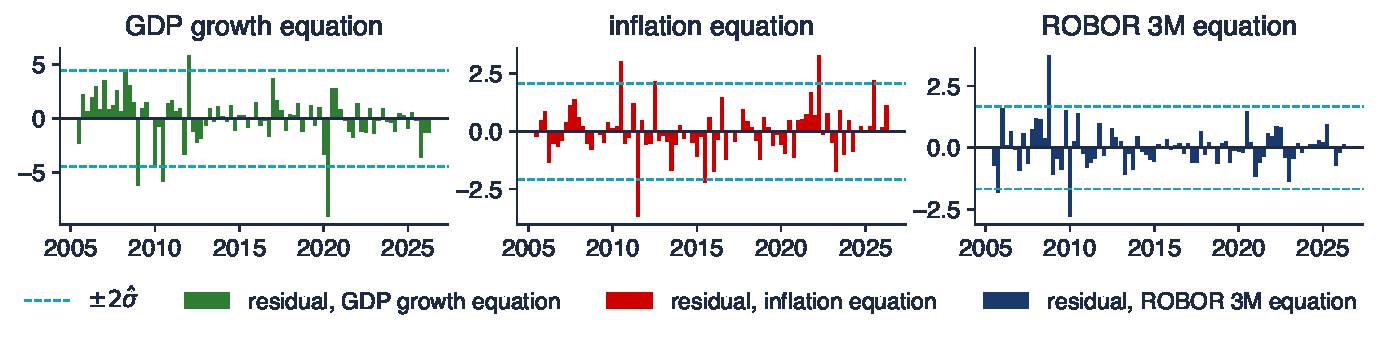
\includegraphics[width=0.97\textwidth,height=0.5\textheight,keepaspectratio]{tsa_ch6_resid.pdf}
\end{center}
\vspace{-0.25cm}
\begin{itemize}
    \item Reziduurile celor trei ecuații, T3 2005--T2 2026, cu $\pm 2$ abateri standard ale reziduurilor
\end{itemize}
\quantlet{TSA\_ch6\_estimation\_diagnostics}{\qlurl{TSA_ch6_estimation_diagnostics}}
\end{frame}

\begin{frame}{Interpretarea reziduurilor}
\itemsize{\small}
\begin{itemize}
    \item Cele mai mari reziduuri: PIB -9{,}1 în T2 2020 (pandemia), ROBOR $+3{,}7$ în T4 2008 (criza de lichiditate din 2008), inflația -3{,}7 în T3 2011
    \begin{itemize}
        \item boltire 6{,}5 ($g$) și 7{,}9 ($i$), față de 3 pentru distribuția Normală: Jarque--Bera 191 (p $<$\,0{,}001)
    \end{itemize}
    \item Portmanteau: $Q_8 = 76{,}7$ ($54$ grade de libertate, p 0{,}023); $Q_{12} = 105{,}3$ ($90$ grade de libertate, p 0{,}130)
    \begin{itemize}
        \item la limită pentru 8 decalaje, acceptabil pentru 12: rămîne o corelație pe termen scurt, în parte din cauza ratelor anuale ale inflației care se suprapun
    \end{itemize}
    \item Consecință: estimările punctuale pot fi folosite, dar intervalele din secțiunile următoare se bazează pe aproximări pentru eșantioane mari; pentru răspunsuri folosim benzi bootstrap
\end{itemize}
\end{frame}

\begin{frame}{Recapitulare: diagnosticarea reziduurilor}
\itemsize{\small}
\begin{itemize}
    \item Testul portmanteau: $H_0$ reziduuri zgomot alb, $\chi^2$ cu $K^2(h - p)$ grade de libertate
    \item Normalitatea nu se verifică în datele macroeconomice: crizele produc valori extreme
    \item Remedii: mai multe decalaje, mai multe variabile, dummy pentru trimestrele de criză
\end{itemize}
\end{frame}


%=============================================================================
\section{Cauzalitatea Granger}
%=============================================================================

\begin{frame}{Cauzalitatea Granger: definiția}
\itemsize{\small}
\begin{columns}[T]
\begin{column}{0.3\textwidth}
\centering

\includegraphics[height=0.44\textheight]{ch3_clive_granger_2008.jpg}\\[1mm]
\imgcap{Clive Granger (1934--2009), Premiul Nobel pentru economie 2003}
\imgcredit{https://commons.wikimedia.org/wiki/File:Clive_Granger_by_Olaf_Storbeck_(3x4_cropped).jpg}{Foto: Olaf Storbeck (2008); CC BY-SA 2.0; Wikimedia Commons}
\end{column}
\begin{column}{0.68\textwidth}
\begin{itemize}
    \item \textbf{Definiție} \refGranger: $x$ \textbf{cauzează în sens Granger} pe $y$ dacă trecutul lui $x$ îmbunătățește prognoza lui $y$ făcută din trecutul lui $y$ (și al celorlalte variabile)
    \begin{itemize}
        \item formal: MSE (mean squared error, eroarea pătratică medie) a prognozei optime pentru $y_{t+1}$ este mai mică atunci cînd folosim $x_t, x_{t-1}, \dots$
    \end{itemize}
    \item O afirmație despre \textbf{predictibilitate}, nu despre cauză și efect
    \begin{itemize}
        \item cauza vine înaintea efectului, dar „înainte” nu înseamnă „din cauza”
    \end{itemize}
    \item Patru cazuri: nicio cauzalitate, $x \to y$, $y \to x$, feedback $x \leftrightarrow y$
\end{itemize}
\end{column}
\end{columns}
\end{frame}

\begin{frame}{Testarea cauzalității Granger într-un VAR}
\itemsize{\small}
\begin{itemize}
    \item Într-un VAR$(p)$, $x$ nu cauzează în sens Granger pe $y$ dacă toți coeficienții lui $x_{t-1}, \dots, x_{t-p}$ din ecuația lui $y$ sînt zero
    \begin{itemize}
        \item VAR(2) cu două variabile: $H_0$: $a_{12}^{(1)} = a_{12}^{(2)} = 0$ în $y_t = c + a_{11}^{(1)}y_{t-1} + a_{12}^{(1)}x_{t-1} + a_{11}^{(2)}y_{t-2} + a_{12}^{(2)}x_{t-2} + \varepsilon_t$
    \end{itemize}
    \item \textbf{Testul $F$}: $F = \dfrac{(RSS_R - RSS_U)/p}{RSS_U/(T - Kp - 1)} \sim F(p, T - Kp - 1)$ în ipoteza $H_0$
    \begin{itemize}
        \item $RSS_U$: suma pătratelor reziduurilor din ecuația lui $y$; $RSS_R$: aceeași sumă fără decalajele lui $x$
    \end{itemize}
    \item \textbf{Testul Wald}: $W = (\mathbf{R}\hat{\boldsymbol{\beta}})'[\mathbf{R}\hat{\mathbf{V}}\mathbf{R}']^{-1}(\mathbf{R}\hat{\boldsymbol{\beta}}) \sim \chi^2(p)$; aici $W = pF$
    \begin{itemize}
        \item $\mathbf{R}$ selectează coeficienții testați, $\hat{\mathbf{V}}$ este covarianța lor estimată; ambele versiuni cer variabile staționare
    \end{itemize}
\end{itemize}
\end{frame}

\begin{frame}{Exemplu rezolvat: cauzează creșterea PIB-ului ROBOR în sens Granger?}
\itemsize{\small}
\begin{itemize}
    \item Ecuația lui $i_t$ din VAR(2) românesc, $T = 84$, $K = 3$, $p = 2$
    \begin{itemize}
        \item nerestricționat (cu $g_{t-1}$, $g_{t-2}$): $RSS_U = 58{,}27$; restricționat (fără ele): $RSS_R = 69{,}27$
    \end{itemize}
    \item $F = \dfrac{(69{,}27 - 58{,}27)/2}{58{,}27/77} = \dfrac{5{,}498}{0{,}7568} = 7{,}26$
    \begin{itemize}
        \item grade de libertate $(2, 84 - 6 - 1) = (2, 77)$; valoarea critică de 5\%: 3{,}12; valoarea p: 0{,}001
    \end{itemize}
    \item \textbf{Decizia}: respingem $H_0$: creșterea PIB-ului din trecut ajută la prognoza ROBOR 3M, dat fiind trecutul inflației și al ROBOR
    \begin{itemize}
        \item compatibil cu o bancă centrală care înăsprește politica atunci cînd economia crește repede
    \end{itemize}
\end{itemize}
\end{frame}

\begin{frame}{Cauzalitatea Granger în VAR(2) românesc}
\itemsize{\small}
\begin{center}
\footnotesize
\begin{tabular}{llrr}
\toprule
\textbf{Cauza} & \textbf{Efectul} & $F$ & \textbf{p} \\
\midrule
creșterea PIB & inflația & 0{,}16 & 0{,}853 \\
creșterea PIB & ROBOR 3M & 7{,}26 & 0{,}001 \\
inflația & creșterea PIB & 2{,}94 & 0{,}059 \\
inflația & ROBOR 3M & 4{,}74 & 0{,}011 \\
ROBOR 3M & creșterea PIB & 4{,}02 & 0{,}022 \\
ROBOR 3M & inflația & 0{,}89 & 0{,}417 \\
\bottomrule
\end{tabular}
\end{center}
\begin{itemize}
    \item Teste $F(2, 77)$ în VAR(2), T3 2005--T2 2026; valoarea critică de 5\%: 3{,}12
    \item Semnificative la 5\%: creșterea PIB $\to$ ROBOR, inflația $\to$ ROBOR, ROBOR $\to$ creșterea PIB
\end{itemize}\quantlet{TSA\_ch6\_granger}{\qlurl{TSA_ch6_granger}}
\end{frame}

\begin{frame}{Interpretarea testelor Granger}
\itemsize{\small}
\begin{itemize}
    \item Dobînda urmează economia: creșterea și inflația din trecut ajută la prognoza ROBOR
    \begin{itemize}
        \item tiparul unei funcții de reacție (banca centrală răspunde la inflație și la activitate); testul singur nu poate demonstra că aceasta este regula BNR
    \end{itemize}
    \item ROBOR nu cauzează inflația în sens Granger (p 0{,}417): nicio dovadă că dobînzile din trecut îmbunătățesc prognoza inflației
    \begin{itemize}
        \item aceasta nu înseamnă că politica monetară este ineficientă: efectul poate fi lent, mic față de zgomot sau deja anticipat
    \end{itemize}
    \item ROBOR $\to$ creșterea PIB (p 0{,}022): dobînzile mai mari preced o creștere mai slabă; în VAR-ul cu două variabile (PIB, ROBOR) valoarea p este 0{,}063
\end{itemize}
\end{frame}

\begin{frame}{Piețe: precedă New York-ul Frankfurtul și Bucureștiul?}
\itemsize{\footnotesize}
\begin{columns}[T]
\begin{column}{0.36\textwidth}
\centering
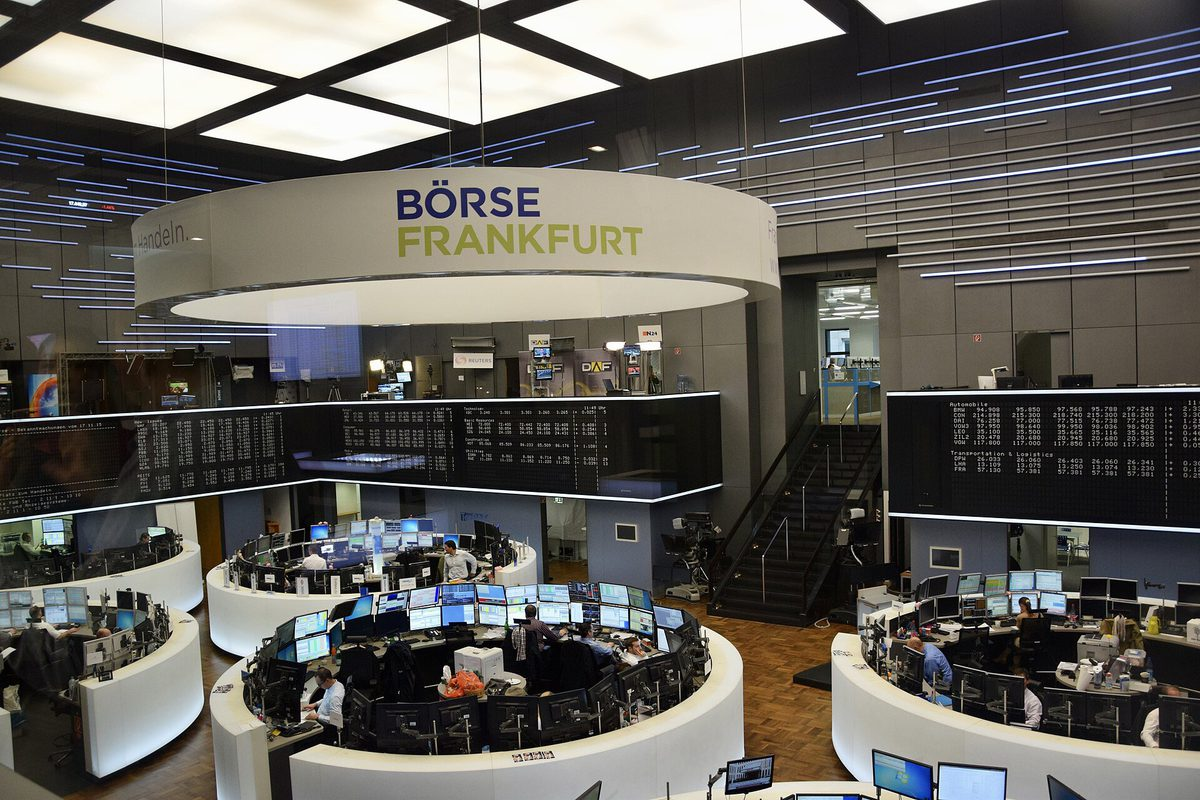
\includegraphics[height=0.34\textheight]{ch6_frankfurt_exchange_2015.jpg}\\[1mm]
\imgcap{Sala de tranzacționare a Bursei din Frankfurt (DAX)}
\imgcredit{https://commons.wikimedia.org/wiki/File:Frankfurt_Stock_Exchange_(Ank_Kumar)_01.jpg}{Foto: Ank Kumar (2015); CC BY-SA 4.0; Wikimedia Commons}
\end{column}
\begin{column}{0.62\textwidth}
\begin{center}
\scriptsize
\begin{tabular}{llrr}
\toprule
\textbf{Cauza} & \textbf{Efectul} & $F$ & \textbf{p} \\
\midrule
S\&P 500 & DAX & 94{,}6 & $<$\,0{,}001 \\
S\&P 500 & BET & 37{,}8 & $<$\,0{,}001 \\
DAX & S\&P 500 & 6{,}9 & $<$\,0{,}001 \\
DAX & BET & 3{,}2 & 0{,}012 \\
BET & S\&P 500 & 1{,}0 & 0{,}416 \\
BET & DAX & 2{,}6 & 0{,}032 \\
\bottomrule
\end{tabular}
\end{center}
\begin{itemize}
    \item Randamente logaritmice zilnice, VAR(4) (ordinul din \refDYb), 6\,429 de zile, 2000--2026; teste $F(4, \cdot)$; HQ ar alege $p = 2$, AIC $p = 8$
    \item Coeficientul S\&P 500 de ieri în ecuația BET: 0{,}218 (SE 0{,}018); în ecuația DAX: 0{,}346
\end{itemize}
\end{column}
\end{columns}
\quantlet{TSA\_ch6\_granger}{\qlurl{TSA_ch6_granger}}
\end{frame}

\begin{frame}{Interpretarea testelor pentru piețe}
\itemsize{\small}
\begin{itemize}
    \item Cauzalitate puternică, într-un singur sens, de la S\&P 500 spre DAX și BET: un randament de 1\% al S\&P 500 ieri adaugă circa 0{,}218\% la BET azi
    \begin{itemize}
        \item BET nu cauzează S\&P 500 în sens Granger (p 0{,}416)
    \end{itemize}
    \item Cauza: orele de închidere (tranzacționare nesincronă), nu o piață lentă
    \begin{itemize}
        \item New York tranzacționează și după închiderea Europei; randamentul S\&P „de ieri” s-a produs parțial cînd Europa era închisă
        \item pe date săptămînale efectul este mult mai slab (Seminarul 6, B2)
    \end{itemize}
    \item Se poate cîștiga din asta? Ați cumpăra la deschiderea Bursei de la București, după ce prețurile s-au ajustat deja: cauzalitatea Granger în prețurile de închidere nu este un profit gratuit
\end{itemize}
\end{frame}

\begin{frame}{Capcana 1: variabilele omise}
\itemsize{\small}
\begin{itemize}
    \item Cauzalitatea Granger depinde de setul de informații: adăugarea sau eliminarea unei variabile o poate crea sau distruge \refLutOm
    \begin{itemize}
        \item un factor comun $z$ care afectează pe $x$ mai devreme decît pe $y$ îl face pe $x$ să pară o cauză a lui $y$
    \end{itemize}
    \item Simulare: $z_t = 0{,}5z_{t-1} + e_t$, $x_t = 0{,}8z_{t-1} + u_t$, $y_t = 0{,}8z_{t-2} + v_t$
    \begin{itemize}
        \item $x$ nu apare niciodată în ecuația lui $y$; dar $x_{t-1}$ este o măsură zgomotoasă a lui $z_{t-2}$, care determină pe $y_t$
    \end{itemize}
    \item Exemplu: vînzările de înghețată cauzează înecurile în sens Granger într-un model cu două variabile; temperatura, factorul omis, le explică pe amîndouă
\end{itemize}
\end{frame}

\begin{frame}{Cauzalitate Granger falsă din cauza unei variabile omise}
\itemsize{\footnotesize}
\begin{center}
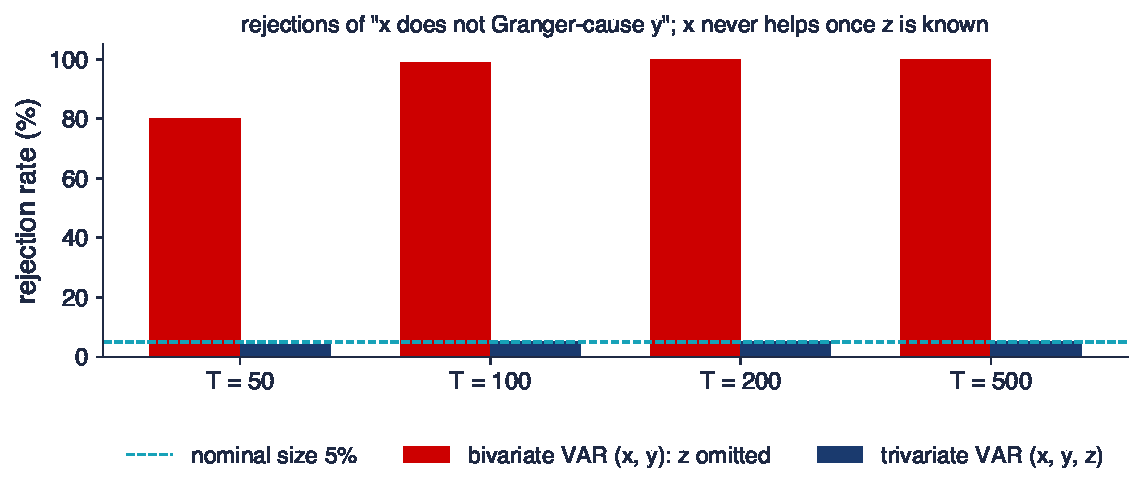
\includegraphics[width=0.97\textwidth,height=0.52\textheight,keepaspectratio]{tsa_ch6_granger_sim.pdf}
\end{center}
\vspace{-0.25cm}
\begin{itemize}
    \item 1\,000 de simulări pentru fiecare volum al eșantionului, cu sistemul de pe slide-ul anterior; testul $F$ pentru „$x$ nu cauzează $y$ în sens Granger” la 5\% într-un VAR(2), cu și fără $z$
\end{itemize}
\quantlet{TSA\_ch6\_granger}{\qlurl{TSA_ch6_granger}}
\end{frame}

\begin{frame}{Interpretarea simulării}
\itemsize{\small}
\begin{itemize}
    \item Fără $z$, testul respinge în 80\% din eșantioane pentru $T = 50$ și în 100\% pentru $T = 200$: aproape mereu o „cauză”
    \begin{itemize}
        \item mai multe date înrăutățesc situația: testul devine tot mai sigur de o concluzie greșită
    \end{itemize}
    \item Cu $z$ în VAR, rata de respingere este 4{,}3\%--5{,}2\%, apropiată de nivelul nominal de 5\%
    \begin{itemize}
        \item cauzalitatea Granger este o proprietate a sistemului ales, nu a lumii
    \end{itemize}
    \item Exemplu românesc: inflația $\to$ creșterea PIB are p 0{,}059 în VAR-ul cu trei variabile și 0{,}173 în cel cu două variabile
\end{itemize}
\end{frame}

\begin{frame}{Capcana 2: cauzalitatea instantanee}
\itemsize{\small}
\begin{itemize}
    \item Testele Granger folosesc doar decalaje; efectele din aceeași perioadă sînt ascunse în corelația șocurilor $\bSigma$
    \begin{itemize}
        \item \textbf{cauzalitate instantanee} între $x$ și $y$: $\Cov(\varepsilon_{xt}, \varepsilon_{yt}) \ne 0$; testată printr-un test Wald pe elementele din afara diagonalei lui $\bSigma$
    \end{itemize}
    \item Nu are \textbf{direcție}: datele nu pot spune dacă $x$ l-a mișcat pe $y$ sau $y$ pe $x$ în cursul trimestrului
    \begin{itemize}
        \item România: șocurile ROBOR sînt corelate instantaneu cu celelalte (p 0{,}041); corelația reziduurilor inflației și ROBOR este 0{,}25
    \end{itemize}
    \item În datele trimestriale, multe efecte reale au loc în cursul trimestrului: un VAR în care nimic nu este semnificativ în sens Granger poate avea totuși legături puternice (secțiunea 7)
\end{itemize}
\end{frame}

\begin{frame}{Capcana 3: trenduri, așteptări și sensul cuvîntului „cauză”}
\itemsize{\small}
\begin{itemize}
    \item \textbf{Variabile nestaționare}: pentru serii $I(1)$, testele $F$ și Wald nu au distribuțiile obișnuite \refSSW
    \begin{itemize}
        \item remedii: testăm pe diferențe (dacă nu există cointegrare) sau abordarea Toda--Yamamoto \refTY: estimăm un VAR$(p + d_{\max})$ în niveluri și testăm doar primele $p$ decalaje
        \item seriile cointegrate cer un VECM: Capitolul 7
    \end{itemize}
    \item \textbf{Așteptările}: prețurile orientate spre viitor se mișcă înaintea evenimentelor pe care le anticipează
    \begin{itemize}
        \item prețurile acțiunilor cauzează PIB-ul în sens Granger, iar prognozele meteo „cauzează” ploaia; niciuna nu este o cauză în sensul obișnuit
    \end{itemize}
    \item Raportăm: „$x$ ajută la prognoza lui $y$, date fiind aceste variabile și acest eșantion”; niciodată „$x$ cauzează pe $y$”
\end{itemize}
\end{frame}

\begin{frame}{Recapitulare: cauzalitatea Granger}
\itemsize{\small}
\begin{itemize}
    \item $x \to y$ (Granger): decalajele lui $x$ îmbunătățesc prognoza lui $y$; test $F$ sau Wald al restricțiilor nule
    \item România: creșterea PIB și inflația $\to$ ROBOR; piețe: S\&P 500 $\to$ DAX, BET (fusurile orare)
    \item Capcane: variabile omise, efecte instantanee, nestaționaritate, așteptări
    \item Cauzalitatea Granger înseamnă predictibilitate, nu cauzalitate
\end{itemize}
\end{frame}


%=============================================================================
\section{Funcții de răspuns la impuls}
%=============================================================================

\begin{frame}{Răspunsurile la impuls și de ce le ortogonalizăm}
\itemsize{\small}
\begin{itemize}
    \item \textbf{Funcția de răspuns la impuls} (IRF): traiectoria lui $Y_{j,t+h}$, $h = 0, 1, 2, \dots$, după un șoc unic în variabila $k$ la momentul $t$
    \begin{itemize}
        \item din forma de medie mobilă: răspunsul la o modificare unitară a lui $\varepsilon_{kt}$ este coloana $k$ a lui $\bPhi_h$
    \end{itemize}
    \item \textbf{Problema}: șocurile sînt corelate ($\bSigma$ nu este diagonală)
    \begin{itemize}
        \item „un șoc al inflației fără niciun șoc al ROBOR” este un experiment pe care datele îl arată rar: cele două șocuri vin de obicei împreună (corelația 0{,}25)
    \end{itemize}
    \item \textbf{Soluția}: rescriem șocurile ca $\bepsilon_t = \mathbf{P}\mathbf{u}_t$, cu $\mathbf{u}_t$ necorelate, de varianță unitară: $\bSigma = \mathbf{P}\mathbf{P}'$
    \begin{itemize}
        \item \textbf{IRF ortogonalizată}: $\boldsymbol{\Theta}_h = \bPhi_h\mathbf{P}$; elementul $(j, k)$: răspunsul lui $Y_j$ la un șoc $u_k$ de o abatere standard
    \end{itemize}
\end{itemize}
\end{frame}

\begin{frame}{Descompunerea Cholesky și ordinea variabilelor}
\itemsize{\small}
\begin{itemize}
    \item \textbf{Cholesky}: matricea unică $\mathbf{P}$, inferior triunghiulară, cu diagonala pozitivă, pentru care $\bSigma = \mathbf{P}\mathbf{P}'$
    \begin{itemize}
        \item exemplu: $\bSigma = \begin{pmatrix} 1 & 0{,}5 \\ 0{,}5 & 1 \end{pmatrix}$: $\mathbf{P} = \begin{pmatrix} 1{,}000 & 0{,}000 \\ 0{,}500 & 0{,}866 \end{pmatrix}$, deoarece $p_{11} = 1$, $p_{21} = 0{,}5/1$, $p_{22} = \sqrt{1 - 0{,}25}$
    \end{itemize}
    \item \textbf{Structura recursivă}: $\varepsilon_{1t} = p_{11}u_{1t}$, $\varepsilon_{2t} = p_{21}u_{1t} + p_{22}u_{2t}$
    \begin{itemize}
        \item prima variabilă nu este mișcată de $u_2$ în aceeași perioadă; a doua reacționează imediat la ambele
        \item întreaga corelație este atribuită variabilei așezate prima
    \end{itemize}
    \item \textbf{Ordinea contează}: cu $y_2$ prima, $\mathbf{P} = \begin{pmatrix} 0{,}866 & 0{,}500 \\ 0{,}000 & 1{,}000 \end{pmatrix}$ (superior triunghiulară în ordinea inițială)
    \begin{itemize}
        \item regula: ordonăm de la variabila cea mai lentă (nu reacționează în aceeași perioadă) la cea mai rapidă; România: creșterea PIB, inflația, ROBOR
    \end{itemize}
\end{itemize}
\end{frame}

\begin{frame}{Exemplu rezolvat: răspunsuri ortogonalizate}
\itemsize{\small}
\begin{itemize}
    \item VAR(1) din secțiunea 2, ordinea $(y_1, y_2)$: $\boldsymbol{\Theta}_0 = \mathbf{P} = \begin{pmatrix} 1{,}000 & 0{,}000 \\ 0{,}500 & 0{,}866 \end{pmatrix}$
    \begin{itemize}
        \item un șoc $u_1 = 1$ mișcă imediat $y_1$ cu 1 și $y_2$ cu 0{,}500; $u_2 = 1$ mișcă doar $y_2$, cu 0{,}866
    \end{itemize}
    \item O perioadă mai tîrziu: $\boldsymbol{\Theta}_1 = \bA\mathbf{P} = \begin{pmatrix} 0{,}600 & 0{,}173 \\ 0{,}500 & 0{,}346 \end{pmatrix}$
    \begin{itemize}
        \item $y_2$ răspunde la $u_1$ cu 0{,}500: $0{,}3 \cdot 1 + 0{,}4 \cdot 0{,}5$, efectul direct $a_{21}$ plus propria persistență
    \end{itemize}
    \item În general $\boldsymbol{\Theta}_h = \bPhi_h\mathbf{P}$; răspunsul \textbf{cumulat} $\sum_{s \le h}\boldsymbol{\Theta}_s$ dă efectul asupra nivelului cînd VAR-ul este în rate de creștere
\end{itemize}
\end{frame}

\begin{frame}{Răspunsurile la impuls ale VAR(2) românesc}
\itemsize{\footnotesize}
\begin{center}
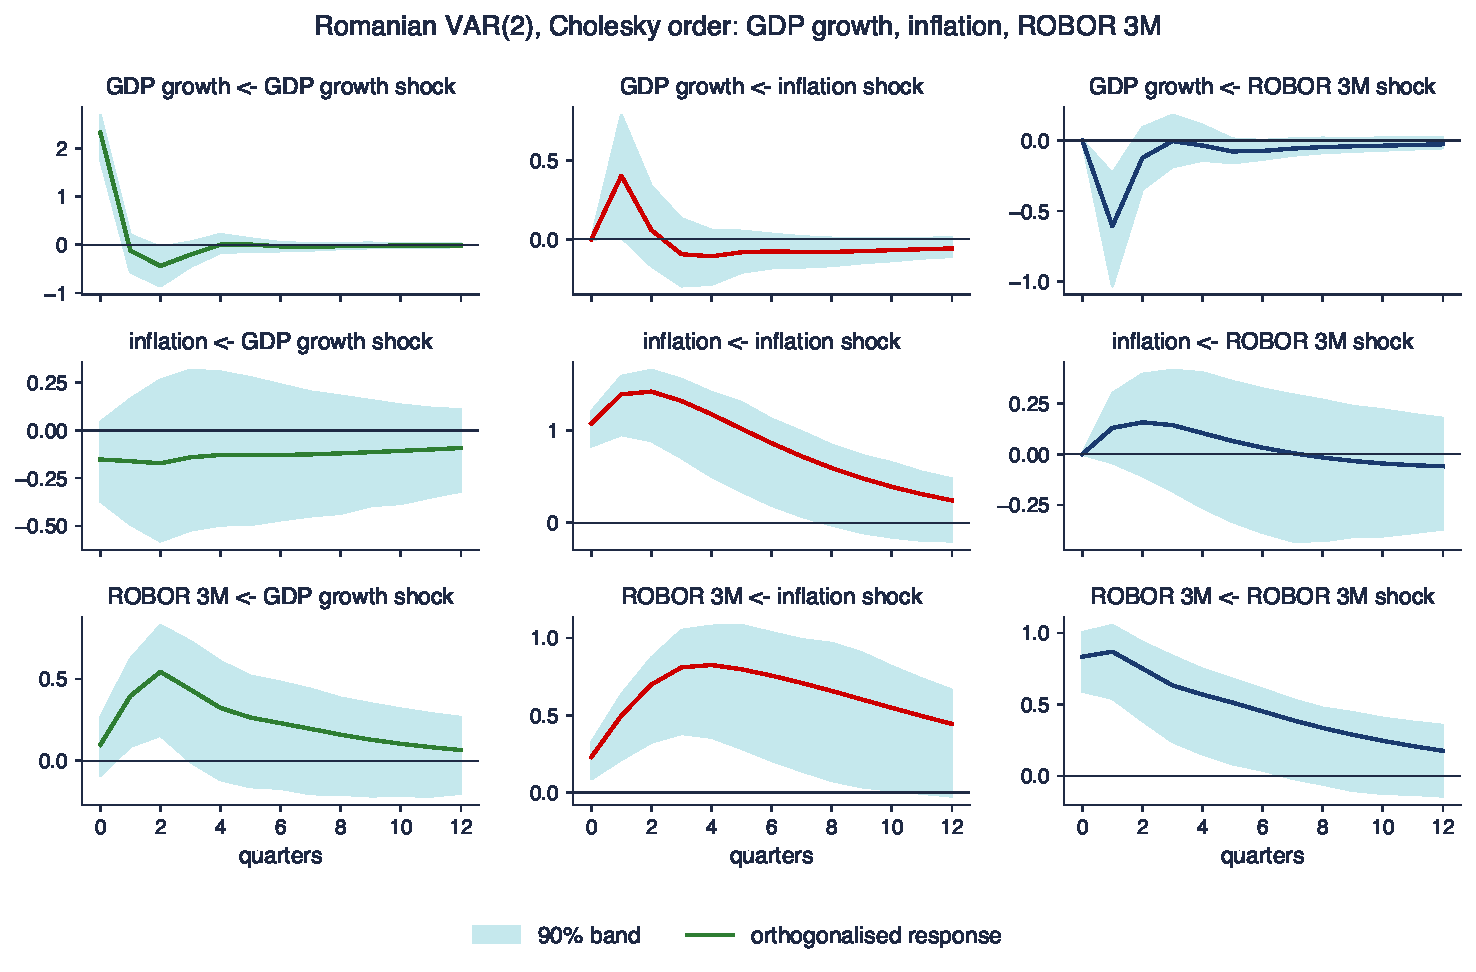
\includegraphics[width=0.97\textwidth,height=0.6\textheight,keepaspectratio]{tsa_ch6_irf_ro.pdf}
\end{center}
\vspace{-0.25cm}
\begin{itemize}
    \item Rîndul: variabila care răspunde; coloana: șocul de o abatere standard; ordinea Cholesky $g, \pi, i$; benzi de 90\% dintr-un bootstrap pe reziduuri (500 de replicări) \refKilian
\end{itemize}
\quantlet{TSA\_ch6\_irf\_fevd}{\qlurl{TSA_ch6_irf_fevd}}
\end{frame}

\begin{frame}{Interpretarea răspunsurilor românești}
\itemsize{\small}
\begin{itemize}
    \item Un șoc al inflației (1{,}08 puncte procentuale la impact) crește ROBOR imediat cu 0{,}23 pp și pînă la 0{,}82 pp după 4 trimestre; încă 0{,}44 pp după 3 ani
    \begin{itemize}
        \item banda exclude zero la 11 din cele 13 orizonturi: cel mai clar rezultat al VAR-ului
    \end{itemize}
    \item Un șoc ROBOR reduce creșterea PIB-ului cu 0{,}61 pp în trimestrul următor, apoi efectul dispare
    \begin{itemize}
        \item dar inflația \textbf{crește} după un șoc ROBOR (pînă la 0{,}16 pp, nesemnificativ): „enigma prețurilor” \refSimsPP
        \item un motiv probabil: dobînda crește atunci cînd banca centrală anticipează inflația; informația omisă din VAR (cursul de schimb, prețurile energiei) apare ca „șoc”
    \end{itemize}
    \item Șocurile inflației sînt persistente: 1{,}18 pp după un an, 0{,}24 pp după trei
\end{itemize}
\end{frame}

\begin{frame}{Schimbă ordinea răspunsul?}
\itemsize{\footnotesize}
\begin{center}
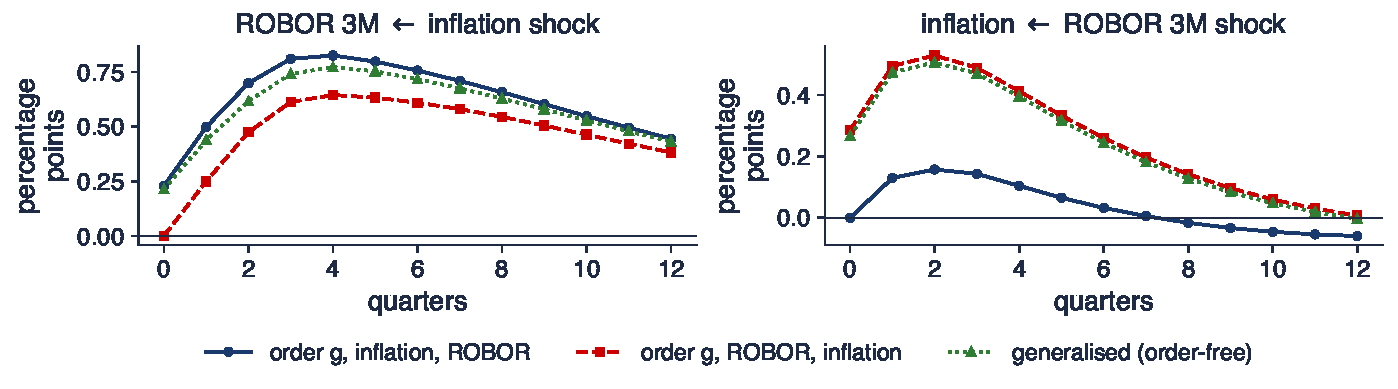
\includegraphics[width=0.97\textwidth,height=0.52\textheight,keepaspectratio]{tsa_ch6_irf_order.pdf}
\end{center}
\vspace{-0.25cm}
\begin{itemize}
    \item Același VAR(2), două ordini Cholesky (inflația înaintea ROBOR, ROBOR înaintea inflației) și răspunsurile generalizate din \refPS, care nu depind de ordine
\end{itemize}
\quantlet{TSA\_ch6\_irf\_fevd}{\qlurl{TSA_ch6_irf_fevd}}
\end{frame}

\begin{frame}{Interpretarea celor două ordini}
\itemsize{\small}
\begin{itemize}
    \item ROBOR după un șoc al inflației: maximul 0{,}82 pp (inflația prima), față de 0{,}64 pp (ROBOR primul)
    \begin{itemize}
        \item cu ROBOR primul, răspunsul la impact este zero prin construcție
    \end{itemize}
    \item Inflația după un șoc ROBOR: 0{,}16 pp, față de 0{,}53 pp, cu 0{,}29 pp deja la impact
    \begin{itemize}
        \item a doua ordine atribuie partea comună a celor două șocuri (corelația 0{,}25) lui ROBOR, deci „enigma prețurilor” crește
    \end{itemize}
    \item Ordinea este o ipoteză despre ce variabilă reacționează în cursul trimestrului; trebuie precizată și justificată, iar rezultatele care se schimbă odată cu ea sînt fragile
\end{itemize}
\end{frame}

\begin{frame}{Răspunsuri la impuls generalizate}
\itemsize{\small}
\begin{itemize}
    \item \textbf{IRF generalizată} \refPS\ (după \refKPP): aplicăm variabilei $k$ un șoc de o abatere standard și lăsăm celelalte șocuri să se miște așa cum se mișcă de obicei odată cu ea
    \begin{itemize}
        \item $\boldsymbol{\psi}_k(h) = \bPhi_h\bSigma\mathbf{e}_k/\sqrt{\sigma_{kk}}$; $\mathbf{e}_k$: coloana $k$ a matricei identitate
    \end{itemize}
    \item Proprietăți
    \begin{itemize}
        \item nu este nevoie de nicio ordine; pentru variabila așezată prima coincide cu răspunsul Cholesky
        \item șocurile nu sînt ortogonale: răspunsurile la șocuri diferite se suprapun și nu se pot aduna
    \end{itemize}
    \item Util pentru piețe, unde nicio ordine nu este naturală; descrie evoluții comune tipice, nu șocuri structurale
\end{itemize}
\end{frame}

\begin{frame}{Piețe: răspunsuri la un șoc S\&P 500}
\itemsize{\footnotesize}
\begin{center}
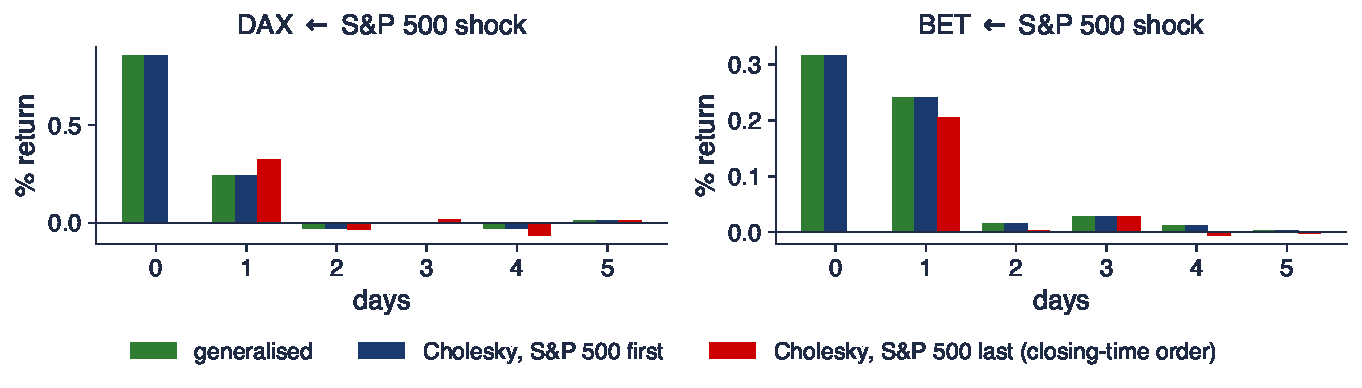
\includegraphics[width=0.97\textwidth,height=0.52\textheight,keepaspectratio]{tsa_ch6_market_irf.pdf}
\end{center}
\vspace{-0.25cm}
\begin{itemize}
    \item VAR(4) al randamentelor zilnice S\&P 500, DAX și BET; șoc S\&P de o abatere standard (1{,}21\%); răspunsuri generalizate, Cholesky cu S\&P 500 primul și Cholesky în ordinea orelor de închidere (BET, DAX, S\&P 500)
\end{itemize}
\quantlet{TSA\_ch6\_market\_spillovers}{\qlurl{TSA_ch6_market_spillovers}}
\end{frame}

\begin{frame}{Interpretarea răspunsurilor piețelor}
\itemsize{\small}
\begin{itemize}
    \item Generalizate: DAX 0{,}85\% în aceeași zi și 0{,}24\% în ziua următoare; BET 0{,}32\% și 0{,}24\%
    \begin{itemize}
        \item identice cu răspunsurile Cholesky cu S\&P 500 primul, cum spune teoria
    \end{itemize}
    \item Cu S\&P 500 ultimul (se închide ultimul), răspunsul din aceeași zi este zero prin ipoteză, iar cele din ziua următoare sînt 0{,}32\% (DAX) și 0{,}20\% (BET)
    \begin{itemize}
        \item corelația din aceeași zi (0{,}63 cu DAX) este atribuită Europei în această ordine
    \end{itemize}
    \item Oricum, efectul dispare după două zile: piețele absorb rapid știrile
\end{itemize}
\end{frame}

\begin{frame}{Recapitulare: funcții de răspuns la impuls}
\itemsize{\small}
\begin{itemize}
    \item IRF: coloanele lui $\bPhi_h$; ortogonalizată: $\boldsymbol{\Theta}_h = \bPhi_h\mathbf{P}$, $\bSigma = \mathbf{P}\mathbf{P}'$
    \item Cholesky = ordine recursivă; ordinea este o ipoteză și poate schimba rezultatele
    \item România: ROBOR crește ani la rînd după un șoc al inflației; apare „enigma prețurilor”
    \item IRF generalizată: nu depinde de ordine, dar nu este aditivă; benzi bootstrap pentru inferență
\end{itemize}
\end{frame}


%=============================================================================
\section{Descompunerea varianței erorii de prognoză}
%=============================================================================

\begin{frame}{Descompunerea varianței erorii de prognoză}
\itemsize{\small}
\begin{itemize}
    \item Eroarea de prognoză la $h$ pași: $\bY_{t+h} - \hat\bY_{t+h|t} = \sum_{s=0}^{h-1}\bPhi_s\bepsilon_{t+h-s} = \sum_{s=0}^{h-1}\boldsymbol{\Theta}_s\mathbf{u}_{t+h-s}$
    \begin{itemize}
        \item șocurile ortogonale $u_k$ sînt necorelate, deci varianța se împarte în $K$ părți
    \end{itemize}
    \item \textbf{FEVD}: $\omega_{jk}(h) = \dfrac{\sum_{s=0}^{h-1}\theta_{jk,s}^2}{\sum_{s=0}^{h-1}\sum_{m=1}^{K}\theta_{jm,s}^2}$, ponderea șocului $k$ în varianța erorii de prognoză la $h$ pași a lui $Y_j$
    \begin{itemize}
        \item fiecare rînd însumează 100\%; depinde de ordinea Cholesky; la $h = 1$ prima variabilă este explicată 100\% de propriul șoc
    \end{itemize}
    \item Exemplu (VAR(1) din secțiunea 2), $h = 2$: varianța erorii pentru $y_2$ este 1{,}37; șocul $u_1$ explică 36{,}5\%
    \begin{itemize}
        \item $(0{,}5^2 + 0{,}5^2)/1{,}37$: impactul $p_{21} = 0{,}5$ și răspunsul din perioada următoare 0{,}500
    \end{itemize}
\end{itemize}
\end{frame}

\begin{frame}{FEVD pentru VAR(2) românesc}
\itemsize{\footnotesize}
\begin{center}
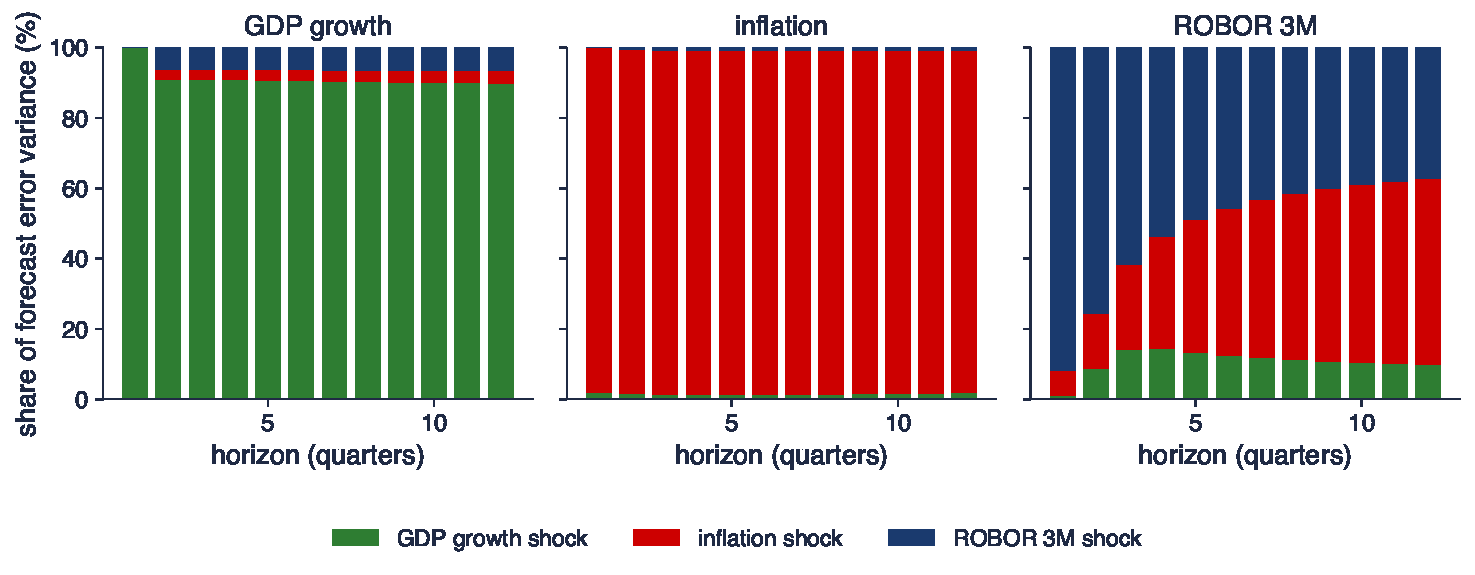
\includegraphics[width=0.97\textwidth,height=0.5\textheight,keepaspectratio]{tsa_ch6_fevd_ro.pdf}
\end{center}
\vspace{-0.25cm}
\begin{itemize}
    \item Ponderea fiecărui șoc ortogonal în varianța erorii de prognoză, orizonturi de 1--12 trimestre, ordinea Cholesky $g, \pi, i$
\end{itemize}
\quantlet{TSA\_ch6\_irf\_fevd}{\qlurl{TSA_ch6_irf_fevd}}
\end{frame}

\begin{frame}{Interpretarea descompunerii varianței}
\itemsize{\small}
\begin{itemize}
    \item ROBOR: propriile șocuri explică 92\% la un trimestru, dar doar 37\% după trei ani; șocurile inflației explică 53\%, cele ale PIB-ului 10\%
    \begin{itemize}
        \item pe termen lung, dobînda este determinată mai ales de inflație
    \end{itemize}
    \item Inflația: 97\% propriile șocuri chiar și după 12 trimestre; creșterea PIB: 90\% propriile șocuri
    \begin{itemize}
        \item în acest VAR mic, inflația este determinată de factori din afara modelului (energie, alimente, curs de schimb, taxe)
    \end{itemize}
    \item FEVD și testele Granger sînt în acord: informația circulă de la inflație și producție spre dobîndă
\end{itemize}
\end{frame}

\begin{frame}{Studiu de caz: Diebold și Yilmaz (2009, 2012)}
\itemsize{\small}
\begin{itemize}
    \item \textbf{Întrebarea}: cît din incertitudinea prognozei unei piețe provine din șocurile altor piețe și cum se schimbă aceasta în timp?
    \begin{itemize}
        \item \refDY: FEVD Cholesky pentru randamentele săptămînale a 19 piețe bursiere; \refDYb: FEVD generalizată, care elimină dependența de ordine
    \end{itemize}
    \item \textbf{Indicele de spillover}: $S(H) = \frac{100}{K}\sum_{j \ne k}\tilde\omega_{jk}(H)$, ponderea medie a șocurilor celorlalte piețe
    \begin{itemize}
        \item $\tilde\omega_{jk}$: FEVD generalizată rescalată astfel încît fiecare rînd să însumeze 1; specificația din \refDYb: VAR(4), $H = 10$ zile, ferestre mobile de 200 de zile
    \end{itemize}
    \item \textbf{Rezultatul}: spillover-ul crește puternic în crize; piețele devin mai conectate exact atunci cînd diversificarea este cea mai necesară
    \begin{itemize}
        \item urmează: indicele pentru S\&P 500, DAX și BET
    \end{itemize}
\end{itemize}
\end{frame}

\begin{frame}{Tabelul de spillover: S\&P 500, DAX, BET}
\itemsize{\small}
\begin{center}
\footnotesize
\begin{tabular}{lrrrr}
\toprule
\textbf{Spre $\leftarrow$ de la (\%)} & S\&P 500 & DAX & BET & \textbf{de la ceilalți} \\
\midrule
S\&P 500 & 69{,}2 & 27{,}1 & 3{,}7 & 30{,}8 \\
DAX & 28{,}2 & 66{,}4 & 5{,}4 & 33{,}6 \\
BET & 7{,}2 & 7{,}5 & 85{,}3 & 14{,}7 \\
\textbf{spre ceilalți} & 35{,}4 & 34{,}6 & 9{,}1 & indice 26{,}4 \\
\bottomrule
\end{tabular}
\end{center}
\begin{itemize}
    \item Rîndul $j$: ponderile varianței erorii de prognoză la 10 zile a pieței $j$ datorate șocurilor din fiecare piață (FEVD generalizată, întregul eșantion 2000--2026)
    \item S\&P 500 primește 27{,}1\% de la DAX, iar DAX 28{,}2\% de la S\&P 500; BET primește 14{,}7\% și transmite doar 9{,}1\%: o piață mică, receptoare netă
\end{itemize}\quantlet{TSA\_ch6\_market\_spillovers}{\qlurl{TSA_ch6_market_spillovers}}
\end{frame}

\begin{frame}{Indicele de spillover în timp}
\itemsize{\footnotesize}
\begin{center}
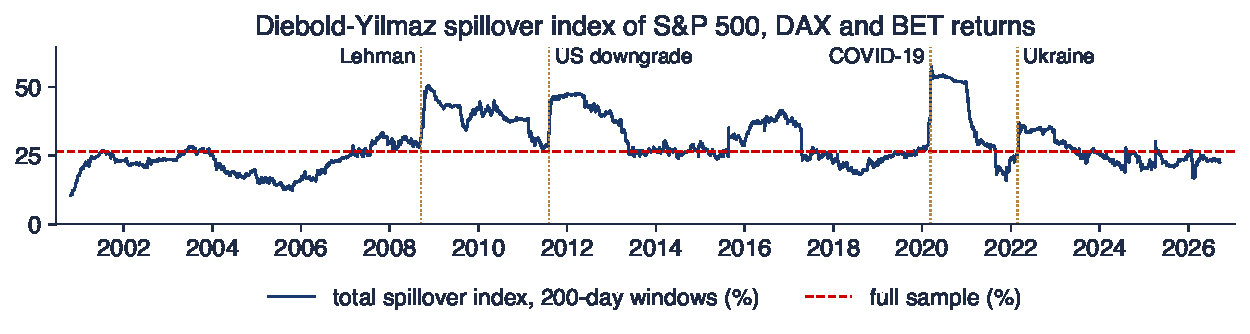
\includegraphics[width=0.97\textwidth,height=0.52\textheight,keepaspectratio]{tsa_ch6_spillover.pdf}
\end{center}
\vspace{-0.25cm}
\begin{itemize}
    \item Indicele total de spillover pentru randamentele zilnice S\&P 500, DAX și BET: FEVD generalizată la 10 zile dintr-un VAR(4), ferestre mobile de 200 de zile de tranzacționare (în medie 29{,}0\%)
\end{itemize}
\quantlet{TSA\_ch6\_market\_spillovers}{\qlurl{TSA_ch6_market_spillovers}}
\end{frame}

\begin{frame}{Interpretarea indicelui de spillover}
\itemsize{\small}
\begin{itemize}
    \item De la 28\% în 2007 la 47\% în T4 2008 (după Lehman); maximul 57{,}5\% pe 17 martie 2020, în prăbușirea din pandemia COVID-19
    \begin{itemize}
        \item același tipar ca în \refDY: conectarea piețelor crește brusc în crize și scade lent
    \end{itemize}
    \item Ultima valoare: 22{,}7\%, sub indicele din întregul eșantion (26{,}4\%)
    \begin{itemize}
        \item salturile sînt în parte mecanice: o fereastră de 200 de zile care conține o prăbușire este dominată de ea timp de 200 de zile
    \end{itemize}
    \item Pentru un portofoliu care conține BET: diversificarea între aceste piețe ajută cel mai puțin atunci cînd este cea mai necesară
\end{itemize}
\end{frame}

\begin{frame}{Recapitulare: descompunerea varianței}
\itemsize{\small}
\begin{itemize}
    \item FEVD: ponderea fiecărui șoc ortogonal în varianța erorii de prognoză la $h$ pași; rîndurile însumează 100\%
    \item România: ROBOR este determinat de inflație pe orizonturi lungi; inflația mai ales de propriile șocuri
    \item Indicele de spillover Diebold--Yilmaz: masa din afara diagonalei a FEVD generalizate
    \item Spillover-ul dintre S\&P 500, DAX și BET atinge maximele în crize (2008, 2020)
\end{itemize}
\end{frame}


%=============================================================================
\section{Prognoza cu un VAR}
%=============================================================================

\begin{frame}{Prognozele VAR și incertitudinea lor}
\itemsize{\small}
\begin{itemize}
    \item \textbf{Prognozele punctuale} prin recurență: $\hat\bY_{T+h|T} = \bc + \bA_1\hat\bY_{T+h-1|T} + \dots + \bA_p\hat\bY_{T+h-p|T}$, cu $\hat\bY_{T+j|T} = \bY_{T+j}$ pentru $j \le 0$
    \begin{itemize}
        \item pentru un VAR stabil ele converg spre media $\boldsymbol{\mu}$ cînd $h$ crește
    \end{itemize}
    \item \textbf{Covarianța erorii}: $\bSigma(h) = \sum_{s=0}^{h-1}\bPhi_s\bSigma\bPhi_s'$; crește cu $h$ spre $\bGamma(0)$
    \begin{itemize}
        \item intervalul de 95\% pentru $Y_j$: $\hat Y_{j,T+h|T} \pm 1{,}96\sqrt{\sigma_{jj}(h)}$ (șocuri Normale; incertitudinea parametrilor este ignorată)
        \item exemplu (secțiunea 2): $\bSigma(2) = \bSigma + \bA\bSigma\bA'$, cu varianțele 1{,}39 și 1{,}37
    \end{itemize}
    \item Aceeași logică precum prognozele ARMA din \tsachlink{https://danpele.github.io/Time-Series-Analysis/RO/Cursuri/capitol2_modele_arma.pdf}{Capitolul 2}, cu matrice în locul numerelor
\end{itemize}
\end{frame}

\begin{frame}{VAR(2) românesc: prognoze pe doi ani}
\itemsize{\footnotesize}
\begin{center}
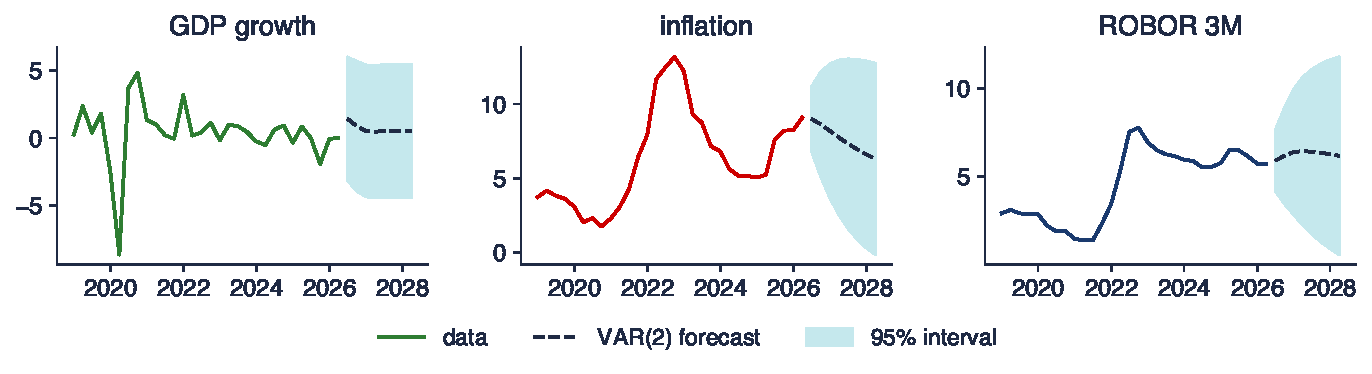
\includegraphics[width=0.97\textwidth,height=0.5\textheight,keepaspectratio]{tsa_ch6_forecast_ro.pdf}
\end{center}
\vspace{-0.25cm}
\begin{itemize}
    \item Date pînă în T2 2026; prognoze pentru T3 2026--T2 2028, cu intervale de 95\%
\end{itemize}
\quantlet{TSA\_ch6\_forecasting}{\qlurl{TSA_ch6_forecasting}}
\end{frame}

\begin{frame}{Interpretarea prognozelor}
\itemsize{\small}
\begin{itemize}
    \item Inflația: de la 9{,}1\% în T2 2026 la 7{,}7\% după un an și 6{,}3\% după doi (95\%: $[-0{,}1; 12{,}7]$)
    \begin{itemize}
        \item prognozele se îndreaptă spre media VAR-ului (inflația 4{,}8\%, ROBOR 4{,}8\%), lent, deoarece cea mai mare valoare proprie este 0{,}869
    \end{itemize}
    \item ROBOR: 6{,}4\% după un an, 6{,}2\% după doi; creșterea PIB: 0{,}5\% pe trimestru, cu intervalul $[-4{,}4; 5{,}3]$
    \begin{itemize}
        \item intervalul PIB-ului este larg pentru că valorile extreme din 2009 și 2020 măresc $\hat\sigma_g$
    \end{itemize}
    \item O prognoză mecanică: nu știe nimic despre buget, prețurile energiei sau deciziile BNR; valoarea ei este aceea de reper transparent
\end{itemize}
\end{frame}

\begin{frame}{Evaluarea corectă a prognozelor VAR}
\itemsize{\small}
\begin{itemize}
    \item \textbf{Pseudo în afara eșantionului}: reestimăm doar pe datele pînă la $t$, prognozăm $t + h$, avansăm $t$ (fereastră care crește)
    \begin{itemize}
        \item nu evaluăm niciodată pe datele folosite la estimare (\tsachlink{https://danpele.github.io/Time-Series-Analysis/RO/Cursuri/capitol0_introducere.pdf}{Capitolul 0})
    \end{itemize}
    \item \textbf{Metode de referință}: mersul aleator (nicio schimbare) și un AR$(p)$ univariat pentru fiecare variabilă, $p$ după AIC
    \begin{itemize}
        \item întrebarea nu este „este VAR-ul bun?”, ci „adaugă ceva celelalte variabile la propriul trecut al seriei?”
    \end{itemize}
    \item Măsuri: RMSE relativ la mersul aleator (sub 1: mai bun); testul Diebold--Mariano \refDM\ pentru acuratețe egală
    \begin{itemize}
        \item statistica DM: media diferenței erorilor pătratice împărțită la eroarea ei standard; aproximativ $N(0, 1)$ în ipoteza $H_0$
    \end{itemize}
\end{itemize}
\end{frame}

\begin{frame}{VAR față de metodele univariate de referință}
\itemsize{\footnotesize}
\begin{center}
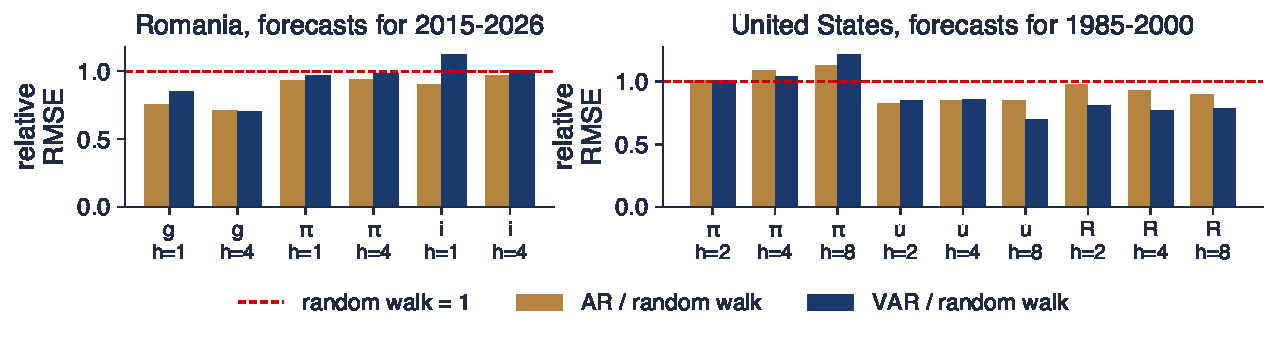
\includegraphics[width=0.97\textwidth,height=0.5\textheight,keepaspectratio]{tsa_ch6_oos.pdf}
\end{center}
\vspace{-0.25cm}
\begin{itemize}
    \item RMSE relativ (model / mers aleator). Stînga: România, 46 de prognoze pe orizont, originile T4 2014--T1 2026; dreapta: VAR-ul american din secțiunea 10, prognoze pentru T1 1985--T4 2000, perioada de evaluare din \refSW
\end{itemize}
\quantlet{TSA\_ch6\_forecasting}{\qlurl{TSA_ch6_forecasting}}
\end{frame}

\begin{frame}{Interpretarea comparației prognozelor}
\itemsize{\small}
\begin{itemize}
    \item România, un trimestru înainte: VAR-ul pierde în fața AR pentru creșterea PIB-ului (0{,}85 față de 0{,}75; DM = 2{,}59, p 0{,}010) și nu este mai bun pentru inflație sau ROBOR
    \begin{itemize}
        \item 21 de coeficienți pe 38--84 de trimestre: zgomotul estimării consumă informația celorlalte variabile
    \end{itemize}
    \item Statele Unite, 8 trimestre înainte: VAR-ul bate AR pentru șomaj (0{,}70 față de 0{,}85) și pentru dobînda federală (0{,}79 față de 0{,}90)
    \begin{itemize}
        \item pentru inflație, nimic nu bate mersul aleator (1{,}22) la acest orizont, în această perioadă
    \end{itemize}
    \item VAR-urile ajută cînd eșantionul este lung și legăturile sînt puternice; în eșantioane scurte și zgomotoase, un AR simplu este greu de depășit
\end{itemize}
\end{frame}

\begin{frame}{Recapitulare: prognoza cu un VAR}
\itemsize{\small}
\begin{itemize}
    \item Prognoze punctuale recursive; covarianța erorii $\sum_s\bPhi_s\bSigma\bPhi_s'$
    \item Evaluăm în afara eșantionului, față de mersul aleator și de modele AR univariate
    \item România: niciun cîștig din VAR; SUA 1985--2000: cîștiguri pentru șomaj și dobîndă
\end{itemize}
\end{frame}


%=============================================================================
\section{VAR-uri structurale și un studiu de caz de referință}
%=============================================================================

\begin{frame}{De la forma redusă la VAR-ul structural}
\itemsize{\small}
\begin{itemize}
    \item \textbf{VAR structural} (SVAR): $\mathbf{B}_0\bY_t = \mathbf{d} + \mathbf{B}_1\bY_{t-1} + \dots + \mathbf{B}_p\bY_{t-p} + \mathbf{u}_t$, $\mathbf{u}_t$ \textbf{șocuri structurale} necorelate
    \begin{itemize}
        \item $\mathbf{B}_0$: efectele contemporane (de exemplu, dobînda de politică monetară reacționează la inflația din acest trimestru)
        \item înmulțind cu $\mathbf{B}_0^{-1}$ obținem forma redusă, cu $\bepsilon_t = \mathbf{B}_0^{-1}\mathbf{u}_t$
    \end{itemize}
    \item \textbf{Identificarea}: $\bSigma$ are $K(K+1)/2$ elemente distincte, $\mathbf{B}_0^{-1}$ are $K^2$; avem nevoie de $K(K-1)/2$ restricții
    \begin{itemize}
        \item Cholesky: $\mathbf{B}_0^{-1} = \mathbf{P}$ inferior triunghiulară: exact $K(K-1)/2$ zerouri; SVAR-ul recursiv din \refSims
        \item alte scheme: restricții pe termen lung, restricții de semn, instrumente externe (dincolo de acest curs)
    \end{itemize}
    \item Datele identifică forma redusă; interpretarea structurală se bazează întotdeauna pe ipoteze care trebuie argumentate economic
\end{itemize}
\end{frame}

\begin{frame}{Studiu de caz: Stock și Watson (2001)}
\itemsize{\footnotesize}
\begin{columns}[T]
\begin{column}{0.4\textwidth}
\centering

\includegraphics[height=0.3\textheight]{ch6_eccles_building_2011.jpg}\\[1mm]
\imgcap{Clădirea Eccles, Washington: Consiliul Rezervei Federale}
\imgcredit{https://commons.wikimedia.org/wiki/File:Eccles_Building_(26088200676).jpg}{Foto: Federal Reserve (2011); public domain; Wikimedia Commons}
\end{column}
\begin{column}{0.58\textwidth}
\begin{itemize}
    \item \refSW: „Vector autoregressions”, o sinteză a metodei, folosită pe scară largă
    \begin{itemize}
        \item trei variabile: inflația (indicele de preț al PIB, $\pi_t = 400\ln(P_t/P_{t-1})$), șomajul, dobînda federală
        \item trimestrial, T1 1960--T4 2000, VAR(4), ordinea Cholesky $\pi, u, R$
    \end{itemize}
    \item Patru sarcini: descrierea datelor, prognoza, inferența structurală, analiza politicilor
    \begin{itemize}
        \item verdictul lor: VAR-urile sînt bune la primele două; ultimele două depind de ipotezele de identificare
    \end{itemize}
    \item Îl reestimăm cu datele FRED de azi (seriile GDPCTPI, UNRATE, FEDFUNDS): cifrele diferă puțin de cele publicate, deoarece datele au fost revizuite
\end{itemize}
\end{column}
\end{columns}
\end{frame}

\begin{frame}{Cele trei serii americane}
\itemsize{\footnotesize}
\begin{center}
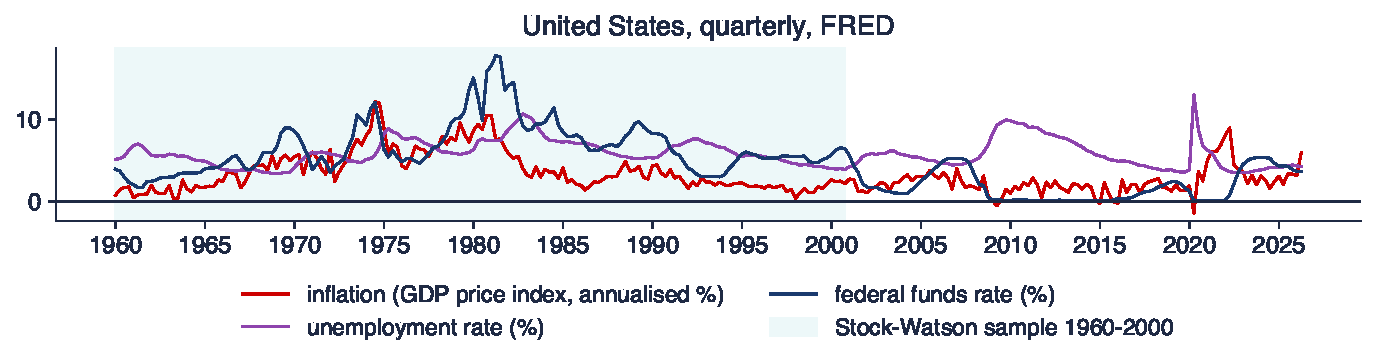
\includegraphics[width=0.97\textwidth,height=0.52\textheight,keepaspectratio]{tsa_ch6_us_data.pdf}
\end{center}
\vspace{-0.25cm}
\begin{itemize}
    \item Trimestrial, T1 1960--T2 2026 (FRED); zona colorată: eșantionul din \refSW, 164 de trimestre
\end{itemize}
\quantlet{TSA\_ch6\_stock\_watson}{\qlurl{TSA_ch6_stock_watson}}
\end{frame}

\begin{frame}{VAR-ul Stock--Watson: răspunsuri la impuls}
\itemsize{\footnotesize}
\begin{center}
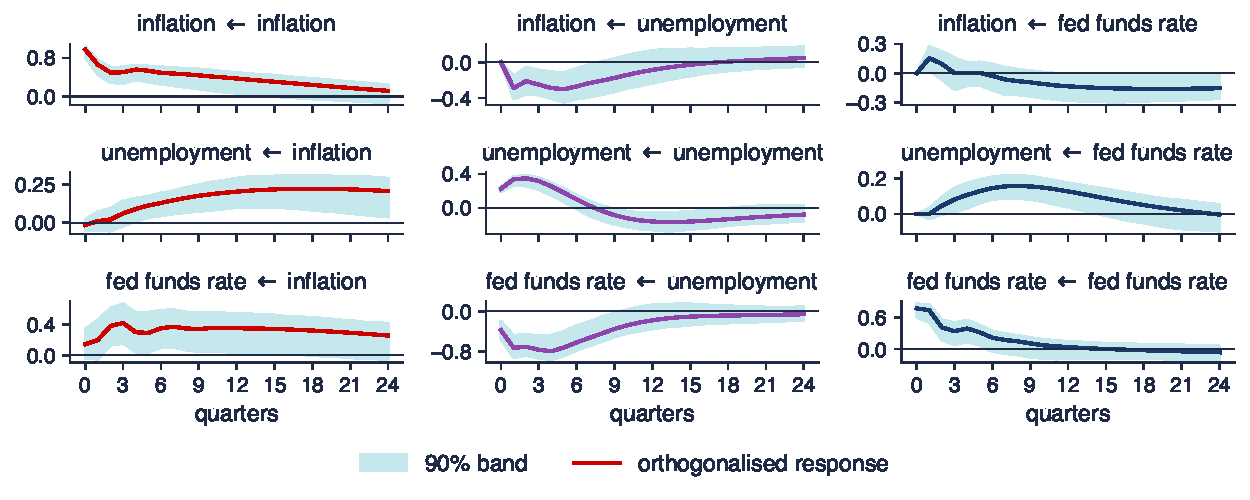
\includegraphics[width=0.97\textwidth,height=0.6\textheight,keepaspectratio]{tsa_ch6_sw_irf.pdf}
\end{center}
\vspace{-0.25cm}
\begin{itemize}
    \item VAR(4), T1 1960--T4 2000, 39 de coeficienți; ordinea Cholesky inflație, șomaj, dobînda federală; 24 de trimestre; benzi bootstrap de 90\%
\end{itemize}
\quantlet{TSA\_ch6\_stock\_watson}{\qlurl{TSA_ch6_stock_watson}}
\end{frame}

\begin{frame}{Interpretarea VAR-ului Stock--Watson}
\itemsize{\small}
\begin{itemize}
    \item Un șoc monetar ($+0{,}78$ pp în dobînda federală) crește șomajul cu pînă la 0{,}16 pp după 8 trimestre
    \begin{itemize}
        \item inflația crește întîi (0{,}16 pp, o enigmă a prețurilor), apoi scade lent (-0{,}13 pp după 3 ani)
    \end{itemize}
    \item Testele Granger: șomajul $\to$ inflația (p 0{,}036), inflația și șomajul $\to$ dobînda federală (p $<$\,0{,}001, $<$\,0{,}001), dobînda federală $\to$ inflația nesemnificativ (p 0{,}402)
    \begin{itemize}
        \item FEVD după 12 trimestre: șocurile monetare explică 19\% din șomaj și 2\% din inflație
    \end{itemize}
    \item Pe eșantionul extins 1960--T2 2026 ($T = 262$) răspunsul șomajului are semnul greșit în primele trimestre (-0{,}13 pp): dobînzile zero de după 2008 și pandemia schimbă sistemul
\end{itemize}
\end{frame}

\begin{frame}{Moștenirea modelului VAR}
\itemsize{\small}
\begin{columns}[T]
\begin{column}{0.5\textwidth}
\centering
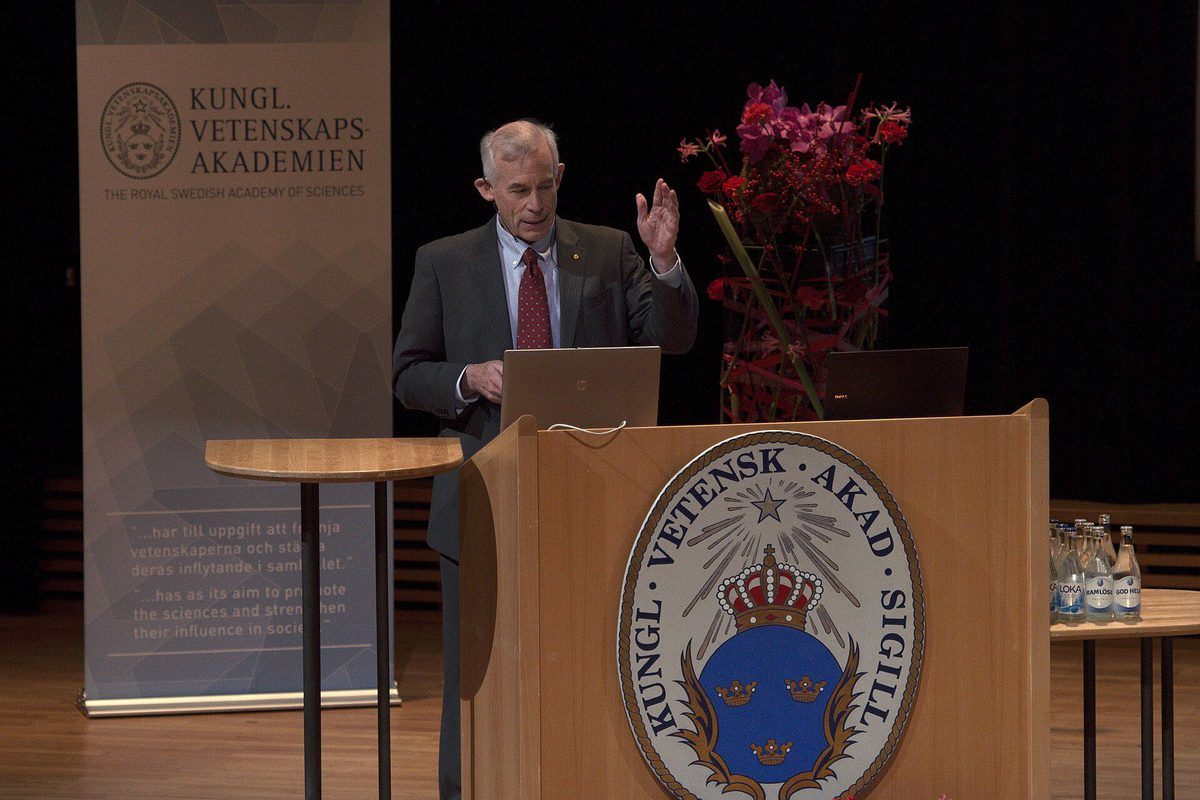
\includegraphics[height=0.4\textheight]{ch6_sims_nobel_lecture_2011.jpg}\\[1mm]
\imgcap{Christopher Sims susținînd prelegerea Nobel, Stockholm, 8 decembrie 2011}
\imgcredit{https://commons.wikimedia.org/wiki/File:Nobel_Prize_2011-Nobel_lectures_KVA-DSC_8085.jpg}{Foto: Holger Motzkau (2011); CC BY-SA 3.0; Wikimedia Commons}
\end{column}
\begin{column}{0.48\textwidth}
\begin{itemize}
    \item Băncile centrale folosesc VAR-uri și modelele derivate din ele (VAR-uri bayesiene, modele DSGE comparate cu VAR-uri) pentru prognoze și scenarii de politică
    \item Enigma prețurilor a dus la adăugarea prețurilor materiilor prime și a așteptărilor în VAR-urile monetare \refSimsPP
    \item Variabilele nestaționare care evoluează împreună cer forma cu corecția erorii: Capitolul 7, cointegrare și VECM \refEG
\end{itemize}
\end{column}
\end{columns}
\end{frame}

\begin{frame}{Recapitulare: VAR-uri structurale}
\itemsize{\small}
\begin{itemize}
    \item SVAR: $\bepsilon_t = \mathbf{B}_0^{-1}\mathbf{u}_t$; $K(K-1)/2$ restricții identifică șocurile structurale
    \item Cholesky este cea mai simplă identificare (recursivă)
    \item Stock și Watson (2001): un șoc monetar crește șomajul; inflația reacționează lent
    \item Rezultatele depind de eșantion și de identificare
\end{itemize}
\end{frame}


%=============================================================================
\section{Contribuția posibilă a AI}
%=============================================================================

\begin{frame}{Contribuția posibilă a AI}
\itemsize{\small}
\begin{itemize}
    \item \textbf{Cod}: o primă versiune a unui script care descarcă mai multe serii, le aliniază datele, alege $p$ și estimează un VAR
    \item \textbf{Explicații}: o a doua explicație a descompunerii Cholesky sau a unui tabel FEVD
    \item \textbf{Explorare}: teste Granger și indici de spillover pentru multe perechi de piețe sau de țări din UE deodată
    \item Exemplu de prompt
    \begin{itemize}
        \item \aiprompt{Write Python code that builds a quarterly data set for Romania (real GDP growth from Eurostat namq\_10\_gdp, 12-month HICP inflation from prc\_hicp\_minr, ROBOR 3M from irt\_st\_m), chooses the VAR lag order by AIC, BIC and HQ, checks stability and residuals, runs Granger tests and plots orthogonalised impulse responses with bootstrap bands.}
    \end{itemize}
\end{itemize}
\end{frame}

\begin{frame}{Verificări necesare}
\itemsize{\small}
\begin{itemize}
    \item Datele calendaristice: serii aliniate pe aceleași trimestre, fără valori completate înainte sau suprapuse care creează precedențe false
    \item Staționaritatea fiecărei variabile (\tsachlink{https://danpele.github.io/Time-Series-Analysis/RO/Cursuri/capitol3_radacini_unitare_modele_arima.pdf}{Capitolul 3}) înaintea testelor Granger; pentru variabile $I(1)$: diferențe, Toda--Yamamoto sau un VECM
    \item Stabilitatea din matricea companion, nu doar din $\bA_1$
    \item Ordinea Cholesky folosită și justificarea ei; aceleași rezultate cu altă ordine sau cu răspunsuri generalizate
    \item Că „cauzează în sens Granger” nu este raportat niciodată drept „cauzează”
    \item Fiecare referință citată: trebuie să existe; verificați DOI-ul
\end{itemize}
\end{frame}


%=============================================================================
\section{Rezumat}
%=============================================================================

\begin{frame}{Idei de reținut}
\itemsize{\small}
\begin{itemize}
    \item Un VAR$(p)$ regresează fiecare variabilă pe trecutul tuturor; OLS ecuație cu ecuație; puține variabile și decalaje
    \item Stabilitatea: toate valorile proprii ale matricei companion în interiorul cercului unitate; atunci există o medie și o formă de medie mobilă
    \item Alegem $p$ cu AIC, BIC, HQ, apoi verificăm reziduurile cu testul portmanteau
    \item Cauzalitatea Granger = predictibilitate suplimentară, relativă la variabilele alese
    \item IRF și FEVD cer șocuri ortogonale: ordinea Cholesky este o ipoteză de identificare
    \item Prognozele VAR trebuie să bată în afara eșantionului metodele AR și mersul aleator; adesea nu reușesc
\end{itemize}
\end{frame}

\begin{frame}{Formule de reținut}
\itemsize{\small}
{\renewcommand{\arraystretch}{1.35}\begin{center}
\scriptsize
\begin{tabular}{ll}
\toprule
\textbf{Mărimea} & \textbf{Formula} \\
\midrule
VAR$(p)$ & $\bY_t = \bc + \bA_1\bY_{t-1} + \dots + \bA_p\bY_{t-p} + \bepsilon_t$, \quad $E[\bepsilon_t\bepsilon_t'] = \bSigma$ \\
Stabilitate, medie & $|\lambda_i(\mathbf{F})| < 1$; \quad $\boldsymbol{\mu} = (\mathbf{I} - \bA_1 - \dots - \bA_p)^{-1}\bc$ \\
Criterii & $\ln\det\tilde\bSigma(p) + c_T\,pK^2/T$, \quad $c_T = 2,\ \ln T,\ 2\ln\ln T$ \\
Portmanteau & $Q_h \sim \chi^2(K^2(h - p))$ \\
Granger $F$ & $\dfrac{(RSS_R - RSS_U)/p}{RSS_U/(T - Kp - 1)} \sim F(p, T - Kp - 1)$ \\
Forma MA, IRF & $\bPhi_h = \sum_{j=1}^{\min(h,p)}\bA_j\bPhi_{h-j}$, \quad $\boldsymbol{\Theta}_h = \bPhi_h\mathbf{P}$, \quad $\bSigma = \mathbf{P}\mathbf{P}'$ \\
FEVD & $\omega_{jk}(h) = \sum_{s<h}\theta_{jk,s}^2 / \sum_{s<h}\sum_m\theta_{jm,s}^2$ \\
Eroarea de prognoză & $\bSigma(h) = \sum_{s=0}^{h-1}\bPhi_s\bSigma\bPhi_s'$ \\
\bottomrule
\end{tabular}
\end{center}
}
\end{frame}

\begin{frame}{Autoevaluare}
\itemsize{\small}
\begin{itemize}
    \item \textbf{Întrebare}: este stabil VAR(1) cu $\bA = \begin{pmatrix} 0{,}9 & 0{,}3 \\ 0{,}2 & 0{,}8 \end{pmatrix}$?
    \begin{itemize}
        \item \textbf{Răspuns}: nu: $\lambda^2 - 1{,}7\lambda + 0{,}66 = 0$ dă $\lambda = 1{,}1$ și $0{,}6$
    \end{itemize}
    \item \textbf{Întrebare}: un test Granger dă p = 0,30 pentru $x \to y$. Nu are $x$ niciun efect asupra lui $y$?
    \begin{itemize}
        \item \textbf{Răspuns}: nu putem concluziona asta: decalajele lui $x$ nu îmbunătățesc prognoza; rămîn posibile efecte în aceeași perioadă, efecte lente sau o putere mică a testului
    \end{itemize}
    \item \textbf{Întrebare}: într-o FEVD Cholesky, ce pondere din varianța erorii la un pas a primei variabile provine din propriul șoc?
    \begin{itemize}
        \item \textbf{Răspuns}: 100\%, prin construcția ordinii
    \end{itemize}
    \item Urmează: Capitolul 7, cointegrarea și modelul vectorial cu corecția erorii (VECM)
\end{itemize}
\end{frame}


%=============================================================================
\section{Bibliografie}
%=============================================================================

\begin{frame}{Bibliografie (1/2)}
\itemsize{\tiny}
\begin{itemize}
    \item Akaike, H. (1974). A new look at the statistical model identification. \textit{IEEE Transactions on Automatic Control}, 19(6), 716--723. \href{https://doi.org/10.1109/TAC.1974.1100705}{doi:10.1109/TAC.1974.1100705}
    \item Diebold, F. X., \& Mariano, R. S. (1995). Comparing predictive accuracy. \textit{Journal of Business \& Economic Statistics}, 13(3), 253--263. \href{https://doi.org/10.1080/07350015.1995.10524599}{doi:10.1080/07350015.1995.10524599}
    \item Diebold, F. X., \& Yilmaz, K. (2009). Measuring financial asset return and volatility spillovers, with application to global equity markets. \textit{The Economic Journal}, 119(534), 158--171. \href{https://doi.org/10.1111/j.1468-0297.2008.02208.x}{doi:10.1111/j.1468-0297.2008.02208.x}
    \item Diebold, F. X., \& Yilmaz, K. (2012). Better to give than to receive: Predictive directional measurement of volatility spillovers. \textit{International Journal of Forecasting}, 28(1), 57--66. \href{https://doi.org/10.1016/j.ijforecast.2011.02.006}{doi:10.1016/j.ijforecast.2011.02.006}
    \item Engle, R. F., \& Granger, C. W. J. (1987). Co-integration and error correction: Representation, estimation, and testing. \textit{Econometrica}, 55(2), 251--276. \href{https://doi.org/10.2307/1913236}{doi:10.2307/1913236}
    \item Granger, C. W. J. (1969). Investigating causal relations by econometric models and cross-spectral methods. \textit{Econometrica}, 37(3), 424--438. \href{https://doi.org/10.2307/1912791}{doi:10.2307/1912791}
    \item Hamilton, J. D. (1994). \textit{Time Series Analysis}. Princeton University Press. \href{https://doi.org/10.2307/j.ctv14jx6sm}{doi:10.2307/j.ctv14jx6sm}
    \item Hannan, E. J., \& Quinn, B. G. (1979). The determination of the order of an autoregression. \textit{Journal of the Royal Statistical Society: Series B}, 41(2), 190--195. \href{https://doi.org/10.1111/j.2517-6161.1979.tb01072.x}{doi:10.1111/j.2517-6161.1979.tb01072.x}
    \item Hosking, J. R. M. (1980). The multivariate portmanteau statistic. \textit{Journal of the American Statistical Association}, 75(371), 602--608. \href{https://doi.org/10.1080/01621459.1980.10477520}{doi:10.1080/01621459.1980.10477520}
    \item Huang, C., \& Petukhina, A. (2022). \textit{Applied Time Series Analysis and Forecasting with Python}. Springer. \href{https://doi.org/10.1007/978-3-031-13584-2}{doi:10.1007/978-3-031-13584-2}
    \item Hyndman, R. J., \& Athanasopoulos, G. (2021). \textit{Forecasting: Principles and Practice} (3rd ed.), Section 12.3, Vector autoregressions. OTexts. \href{https://otexts.com/fpp3/VAR.html}{otexts.com/fpp3/VAR.html}
    \item Jarque, C. M., \& Bera, A. K. (1980). Efficient tests for normality, homoscedasticity and serial independence of regression residuals. \textit{Economics Letters}, 6(3), 255--259. \href{https://doi.org/10.1016/0165-1765(80)90024-5}{doi:10.1016/0165-1765(80)90024-5}
    \item Kilian, L. (1998). Small-sample confidence intervals for impulse response functions. \textit{Review of Economics and Statistics}, 80(2), 218--230. \href{https://doi.org/10.1162/003465398557465}{doi:10.1162/003465398557465}
    \item Koop, G., Pesaran, M. H., \& Potter, S. M. (1996). Impulse response analysis in nonlinear multivariate models. \textit{Journal of Econometrics}, 74(1), 119--147. \href{https://doi.org/10.1016/0304-4076(95)01753-4}{doi:10.1016/0304-4076(95)01753-4}
    \item Lütkepohl, H. (1982). Non-causality due to omitted variables. \textit{Journal of Econometrics}, 19(2--3), 367--378. \href{https://doi.org/10.1016/0304-4076(82)90011-2}{doi:10.1016/0304-4076(82)90011-2}
    \item Lütkepohl, H. (2005). \textit{New Introduction to Multiple Time Series Analysis}. Springer. \href{https://doi.org/10.1007/978-3-540-27752-1}{doi:10.1007/978-3-540-27752-1}
\end{itemize}
\end{frame}

\begin{frame}{Bibliografie (2/2)}
\itemsize{\tiny}
\begin{itemize}
    \item Pesaran, M. H., \& Shin, Y. (1998). Generalized impulse response analysis in linear multivariate models. \textit{Economics Letters}, 58(1), 17--29. \href{https://doi.org/10.1016/S0165-1765(97)00214-0}{doi:10.1016/S0165-1765(97)00214-0}
    \item Schwarz, G. (1978). Estimating the dimension of a model. \textit{The Annals of Statistics}, 6(2), 461--464. \href{https://doi.org/10.1214/aos/1176344136}{doi:10.1214/aos/1176344136}
    \item Sims, C. A. (1980). Macroeconomics and reality. \textit{Econometrica}, 48(1), 1--48. \href{https://doi.org/10.2307/1912017}{doi:10.2307/1912017}
    \item Sims, C. A. (1992). Interpreting the macroeconomic time series facts: The effects of monetary policy. \textit{European Economic Review}, 36(5), 975--1000. \href{https://doi.org/10.1016/0014-2921(92)90041-T}{doi:10.1016/0014-2921(92)90041-T}
    \item Sims, C. A., Stock, J. H., \& Watson, M. W. (1990). Inference in linear time series models with some unit roots. \textit{Econometrica}, 58(1), 113--144. \href{https://doi.org/10.2307/2938337}{doi:10.2307/2938337}
    \item Stock, J. H., \& Watson, M. W. (2001). Vector autoregressions. \textit{Journal of Economic Perspectives}, 15(4), 101--115. \href{https://doi.org/10.1257/jep.15.4.101}{doi:10.1257/jep.15.4.101}
    \item Toda, H. Y., \& Yamamoto, T. (1995). Statistical inference in vector autoregressions with possibly integrated processes. \textit{Journal of Econometrics}, 66(1--2), 225--250. \href{https://doi.org/10.1016/0304-4076(94)01616-8}{doi:10.1016/0304-4076(94)01616-8}
\end{itemize}
\end{frame}

\end{document}
